% !Mode:: "TeX:UTF-8"
\baselineskip 20pt
%-------------------------------------------------------------------------
%\chapter{个性化信息感知的评论摘要生成}
\chapter{融合节点流行度的动态网络建模及层次异常检测}
\label{chap:5}

%上一章提出了针对动态网络节点的社团转移异质性的层次贝叶斯建模方法HB-DSBM,并利用变分推断进行了模型参数求解,通过真实数据的社团检测任务证明了所设计的层次狄利克雷生成结构有效地建模了以社团为介观结构的动态网络生成机制,并从社团到节点的生成机制设计建模了节点的社团演化异质性。HB-DSBM的节点社团转移异质性的生成机制设计主要从生成的角度构建了从社团到节点的社团转移倾向的层次狄利克雷分布,并未与节点本身的特征直接建模,这对动态网络后续分析会造成一定困难。另外,生成模型从网络生成的角度对动态网络进行建模,其本质是刻画了网络的生成和演化机制,因此此类模型应该能够适配大部分下游任务,而HB-DSBM所提出的节点演化异常指数无法直接评估社团、网络在演化层面的异常。
本章将针对动态网络高阶生成机理显式建模问题进一步完善基于动态随机块模型的动态网络建模方法,使其能够刻画节点拓扑及演化异质性,并从演化分析能力提升层面提出针对动态网络的演化异常检测任务提出涵盖动态网络快照-社团-节点的异常检测方法,在真实数据集中进行了应用,以验证本章提出的方法在动态网络建模与应用的有效性。



\section{引言\label{chap5:intro}}

生成模型通过设计动态网络的生成机制,刻画了复杂系统从宏观到微观的生成和演化模式,而社团作为动态网络生成机制中的介观结构,承载了对动态网络生成机制建模的重要角色\cite{ghoshal2021influence},在对动态网络生成机制建模过程中起到承上启下作用,融入社团结构的生成模型往往能够刻画动态网络更加深层次的演化模式。例如,动态随机块模型在对网络进行建模后,可以通过社团归属参数对动态网络社团演化进行分析,挖掘所检测社团的扩张、收缩等时序变化\cite{yang2011detecting}。这使得该模型成为经典的复杂网络生成模型之一而获得了部分研究者的青睐。

近年来,部分研究者针对随机块模型在静态网络中存在的问题进行了改进。例如,针对经典随机块模型对网络中节点异质性建模缺失问题所提出的度修正随机块模型DCSBM\cite{ma2021determining}通过引入节点的度对网络中节点的连边概率进行修正;针对动态随机块模型的重叠社团建模缺失问题所提出的混合随机块模型MMSB\cite{godoy2016accurate}通过提出混合参数来刻画节点属于多个社团的场景。也有研究者考虑随机块模型在不同类型网络中的应用对其进行扩展,例如对属性网络进行适配的NEMBP算法\cite{he2017joint}、对超图进行适配的DCHSBM算法\cite{10214123}等进行适应性的改进与推理等。

上述方法并不适配动态网络,未考虑针对动态网络时序变化进行建模。Yang等人针对动态网络首先提出了动态随机块模型DSBM\cite{yang2011detecting},其改进自经典随机块模型SBM,并引入社团转移矩阵来建模动态网络节点的社团划分随时间的变化;Tang等人107则引入了狄利克雷过程来实现对动态随机块模型的模型选择,即自动确定社团个数;dMMSB\cite{xing2010state}则通过引入逻辑正态先验将混合随机块模型扩展到了动态网络;PDC-SBM\cite{riverain2023poisson}则考虑了动态网络边生成过程中的度异质性问题,引入了度修正参数以提升模型对动态网络的建模精度。

上述方法从经典随机块模型出发,在建模能力与适用性方面将随机块模型进行了改进,但依然存在一定缺陷。首先,在建模能力方面虽然以PDC-SBM为代表的方法从节点度异质性层面建模了动态网络中的节点异质性,但从前文的数据挖掘工作中可以看出,节点的度异质性并不适用所有网络;其次,以DCHSBM为代表的方法从网络类型适用性方面提升随机块模型的应用能力,但并未从任务层面对随机块模型进行扩展,最具代表性的任务即为异常检测。


%已有的方法仅验证模型建模方面的贡献,而忽略了生成模型本身对下游任务的通用性,即使验证了,也忽略了重要的下游任务---异常检测。
异常检测是数据挖掘和模式识别的重要任务之一~\cite{chandola2009anomaly,he2024diffusion},其目的就是寻找数据的正常模式中隐藏的不常见模式,即“离群点”。异常检测吸引了大量研究,并已广泛应用于多个领域,如欺诈检测~\cite{ahmed2016survey}和异常行为检测~\cite{amraee2018anomaly}。因此,近年来提出了多种方法。由于复杂网络可以用于建模众多现实世界系统,从国际航空运输~\cite{kasai2016network}到团队协作网络~\cite{dai2024gated},从社交网络~\cite{singh2024social}到引用网络~\cite{yan2024modeling},近年来,网络异常检测也受到了广泛关注,成为当前研究中的关键问题之一。与一般的异常检测类似,但有所超越,复杂网络中的异常检测通常指的是寻找那些模式显著偏离网络绝大多数节点的节点~\cite{lim2024future,li2024unsupervised},或是触发网络在不同层次(即微观层次、中观层次和宏观层次)发生显著结构变化的节点~\cite{hayat2024deep}。



由于网络结构本身随时间演化(动态或时间网络)\cite{huang2015triadic},例如节点的增加和消失以及边的变化,这些因素也驱动了社团的动态行为。因此,确定动态网络中的变化是正常还是异常变得非常困难。网络异常的原因也非常复杂,异常的形式多种多样,包括异常节点、异常边、异常子图以及变化点检测\cite{ranshous2015anomaly}。与此同时,动态网络中的异常检测有助于更好地理解网络的演化状态,评估网络的异常程度及其影响,并制定有效的干预措施来应对网络中的潜在危机。例如,通过适当使用异常检测来发现由网络演化引起的非平稳演化时间点,可以提高社团检测的准确性。它还可以应用于生物系统中的异常基因识别、气候预测和金融市场等领域。

一般来说,大多数现有的异常检测方法通常基于特定的视角,即分别在宏观、微观和中观层次上追踪动态网络在不同时间的演化,忽略了这三个层次上异常的相互影响。例如,FALCON~\cite{10597831} 聚焦于微观层次的异常检测(即异常节点或边),QRDN-ZNN~\cite{LI2025107412} 聚焦于神经网络的异常检测,以改进收敛性能,TCDformer~\cite{wan2024tcdformer} 聚焦于宏观层次的异常检测(即变化点)。事实上,在网络演化过程中,多个类型的异常同时发生是很有可能的,并且不同层次上的异常之间是相关的,在一个层次上的异常检测也有助于其他层次上的异常检测。以金融市场中的异常检测为例。在一个金融交易网络中,节点是账户,边是账户之间的交易。那么,微观层次的异常事件可以是与不同社团频繁交易的节点。在现实生活中,该账户可能是正常账户,也可能是用于欺诈的账户。


在中观层次上,异常事件可以是一些账户之间频繁交易,随后突然分裂成两个或更多的群体。这些账户在现实生活中可能属于一个大型公司,这一分裂事件可能表明该公司已经进行了重组。在宏观层次上的异常事件是整个市场发生了剧烈波动,这在金融市场网络中表现为网络变化的一个节点。此外,异常账户的积累可能导致账户群体发生剧变,整个市场的大事件可能会影响所有账户群体和账户(如金融危机)。如图~\ref{fig:example}所示,网络中节点$v_{7}$的状态随时间不断变化,因此它可以被视为整个网络演化中的异常点。换句话说,它的异常导致了整个网络的异常。然而,$v_{7}$的异常也可以视为中观层次异常的结果(即社团的分裂和合并)。这导致了网络演化过程中微观层次(异常节点)和中观层次(异常子图)异常的耦合。因此,可以看出,不同层次的异常之间是有相关性的,在一个层次上的异常检测也有助于其他层次上的异常检测。仅仅考虑单一类型的异常不足以支持网络演化规律的全面挖掘。换言之,网络在宏观、微观和中观层次上的异常是相互关联的,并且受到更深层次因素的驱动。异常只是表象,背后的本质尚未揭示。

\begin{figure}[htbp]
    \centering
    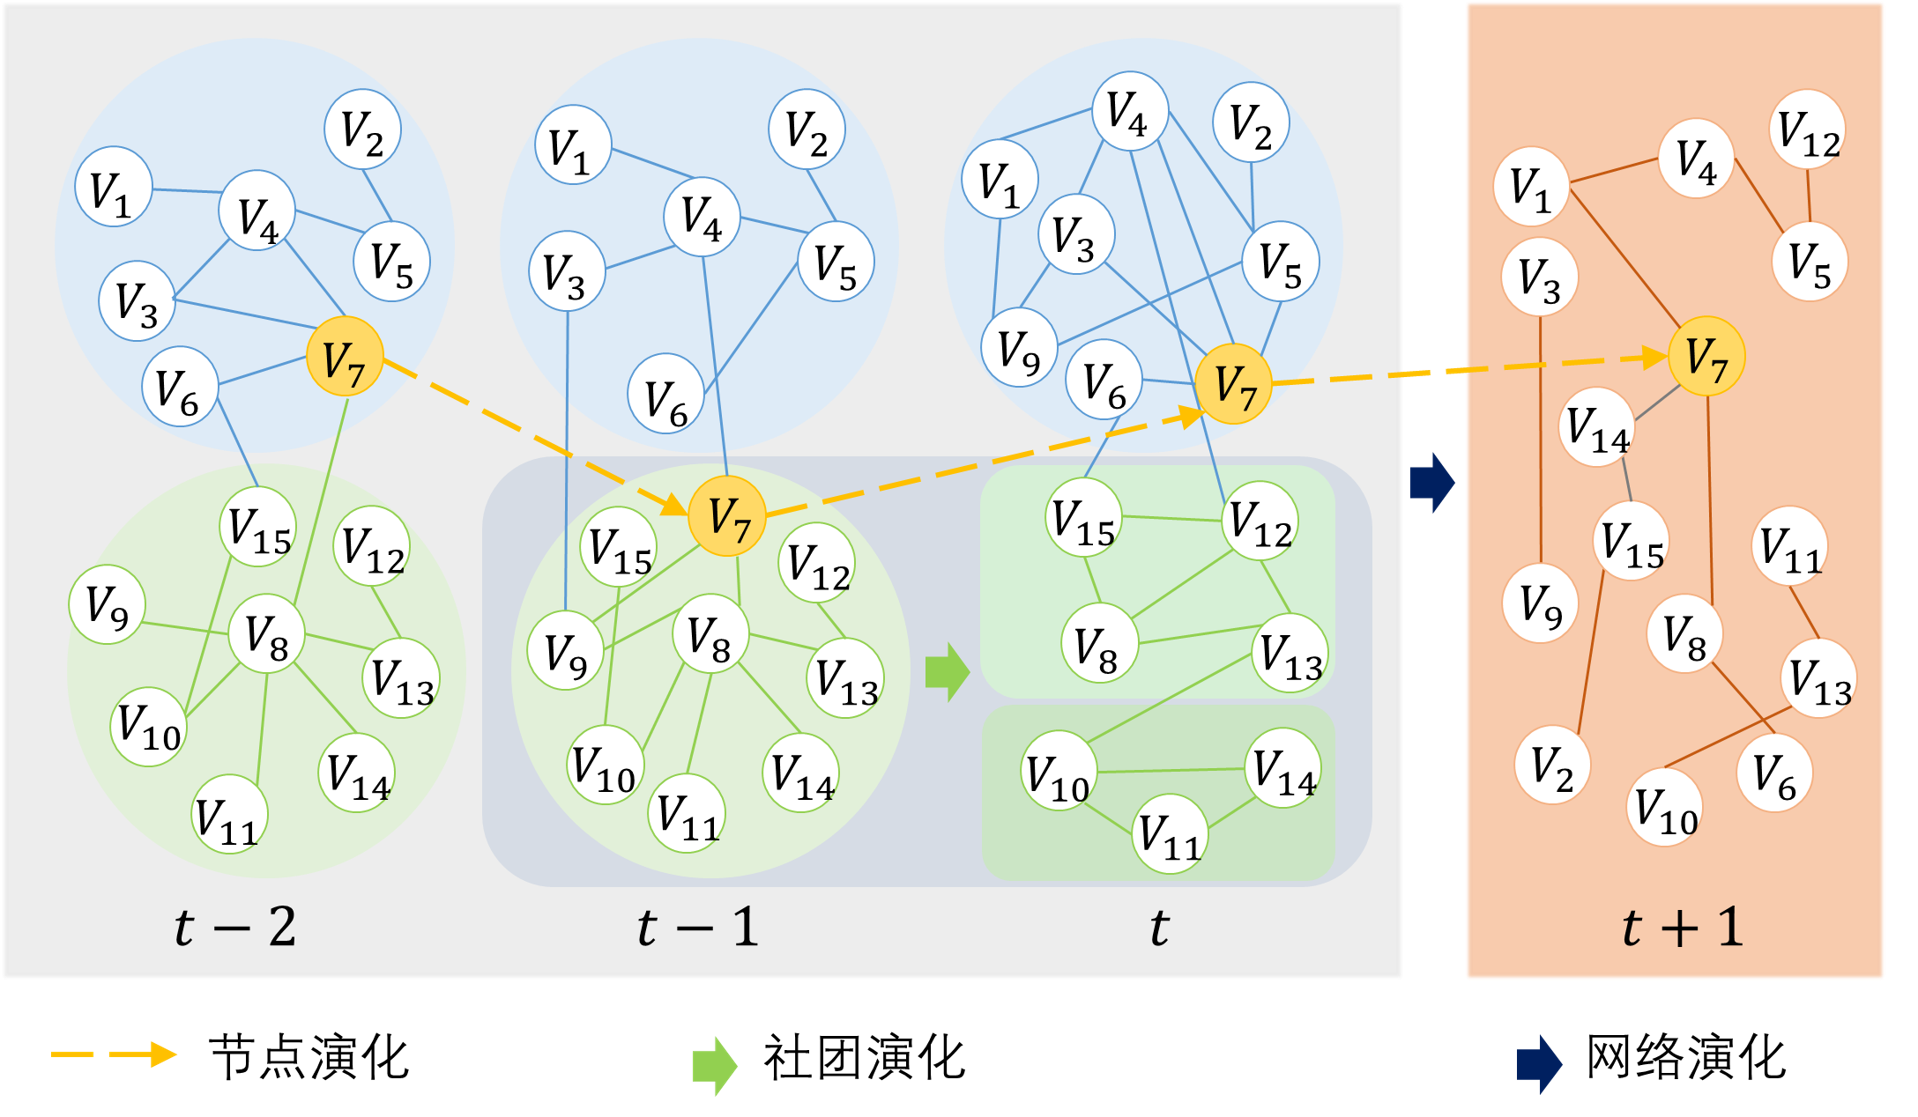
\includegraphics[width=.85\linewidth,trim=0.1in 0.5in 0.1in 0.1in]{figures/chap05/chap5motivation.png}
    \caption{动态网络各层次演化异常样例}
    \label{fig:example}
\end{figure} 





只有少数启发式方法考虑了不同层次异常之间的相关性,例如SCOUT~\cite{hulovatyy2016scout}和MDL~\cite{cheung2020simultaneous}同时检测社团结构异常和网络快照变更点。然而,它们仅考虑了部分而非所有层次的异常,且有些方法需要手动定义特征。此外,这些方法没有统一的框架,它们通过逐步实现不同层次的异常检测,无法建模异常之间的耦合关系,也无法实现异常之间的相互增强。为了捕捉不同层次异常之间的相关性,并更好地检测节点、社团、网络快照的异常,本章采用了统一的生成模型来建模动态网络,以探索不同尺度的异常行为~\cite{wang2019nodes,cheng2008robust}。 

% 异常检测是xxxx 接下面的

% 前文描述的HB-DSBM存在xxx问题,因此本文基于该模型设计了动态网络层次建模方法GEABS并提出了基于该模型参数的异常检测插件,扩展了该模型的下游应用。

% 另一方面,动态网络生成模型建模了网络在生成与演化过程中的复杂机制,此类模型能够支撑动态网络的多种下游任务。例如,前文描述的HB-DSBM模型中,通过拟合社团归属$z$的先验分布$Mult(\pi)$,即可确定网络中任意节点的社团划分;拟合模型中的伯努利分布$Bernoulli(·|B)$,即可预测网络中任意两个节点的边。然而对于网络中的
具体而言,本方法利用生成模型良好的可解释性来探讨异常的本质。本章将节点的流行度、社团成员关系等参数表示为随机块模型(SBM),通过节点流行度来刻画动态网络中节点的异质性,并基于模型参数设计了节点-社团-网络多层异常的检测指标,依次扩展随机块模型在动态网络中任务层面的适用范围。

本章的主要贡献可以概括如下:


\begin{itemize} 
    \item[$\bullet$] 本章提出基于随机块模型的动态网络建模方法GEABS(\textbf{G}eneration model to analyze the dynamic network for \textbf{E}xploring the \textbf{A}bnormal \textbf{B}ehaviors of different \textbf{S}cales),该方法通过建模动态网络节点-社团-网络快照的层次演化模式,并融入节点流行度参数刻画了节点的动态演化行为与拓扑异质性,以提升模型对于动态网络的建模能力。
    \item[$\bullet$] 利用熵与高阶距离度量等指标,结合模型刻画的网络参数,分别设计了网络 、社团、节点的多层次异常检测指标,扩展了本模型的动态网络演化分析能力。
    \item[$\bullet$] 采用变分推断来实现高效的优化。本模型具有良好的通用性,可以轻松应用于各种生成模型,并且其参数均具备一定物理或数学意义,因此具有良好的可解释性。 
    \item[$\bullet$] 实验结果表明,所提出的模型在合成数据集和真实网络中相比于现有的最先进方法,显著提高了动态网络演化分析的性能。
\end{itemize}


\section{融合节点流行度的动态随机块模型描述\label{chap4:model}}

\label{sec:method}
本节首先介绍模型问题定义及参数介绍,随后详细介绍本文提出的动态网络生成模型的架构及其参数后验推断过程。


\subsection{准备工作}
给定一个动态网络 $G =\{ G^{(1)}, G^{(2)}, \cdots, G^{(T)} \}$,每个 $G^{(t)} (1 \le t \le T)$ 是在时间 $t$ 的快照网络。这里记 $N^{(t)}$、$K^{(t)}$ 和 $W^{(t)}$ 分别为快照网络 $G^{(t)}$ 的节点数、社团数和邻接矩阵。为了方便推断与理解,本章假设 $N^{(t)} = N$ 随时间 $t$ 保持不变,而 $W^{(t)}$ 和 $K^{(t)}$ 随时间变化。如果网络是无向无权的,当节点 $V_i$ 和 $V_j$ 在快照 $t$ 上有边时,记 $W^{(t)}_{ij} = 1$ ;否则 $W^{(t)}_{ij} = 0$。为了方便叙述,本文假设动态网络为无向无权网络,但可以很容易地扩展到加权或有向网络(通过将连边概率矩阵$B$约束为非对称矩阵或更改连边概率为泊松分布)。

对于动态网络 $G$,记社团结构为 $Z = \{ Z^{(1)}, Z^{(2)}, \cdots, Z^{(T)} \}$。这里 $Z^{(t)} \in \{0, 1 \}^{K_t \times K_t}$,且 $Z^{(t)}_{ik} = 1$ 表示节点 $V_i$ 属于社团 $k$,$K_t$ 是快照 $t$ 的社团数。在本模型中,只考虑非重叠社团,即 $\sum_{k=1}^{K_t} Z^{(t)}_{ik} = 1$。此外,为了方便,也记 $z^{(t)}_{i} = k$ 代替 $Z^{(t)}_{ik} = 1$。



基于上述内容设置,本章致力于发现网络中的异常模式,形式化如下:
\begin{itemize}
    \item \textbf{宏观层面(网络异常)}:通常与网络变更点相同,即本章找到一个集合 $\mathcal{t} = \{t : |f(G^{(t-1)}) -f(G^{(t)})| > \epsilon  \} $,其中$f$ 是快照网络上的一个映射,$\epsilon$是预定义的阈值。
    \item \textbf{中观层面(社团异常)}:如果社团结构 $Z^{(t-1)}$ 和 $Z^{(t)}$ 有显著差异,意味着存在社团事件,例如社团增长和收缩、合并和分裂等。
    \item \textbf{微观层面(节点异常)}:基于社团成员关系 $Z = \{ Z^{(1)}, Z^{(2)}, \cdots, Z^{(T)} \}$,如果一个节点频繁改变其社团归属,它在动态网络中应被视为异常。
\end{itemize}

在这里,本章将这些问题称为动态网络中的演化异常。网络层面的异常易于分析和评估,但后两个异常难以量化。在本章的GEABS模型中,将从生成模型与社团检测的角度给出网络演化异常的具体定义并进行检测。
本文涉及的主要符号总结在附录A.1~表~\ref{symbols:all} 中。

\subsection{模型的生成过程}

本节将详细介绍GEABS模型的生成过程。对于一个动态网络,它由两部分组成,即网络快照 $t=1$ 和 $t \ge 2$。

\subsubsection{在$G^{(1)}$中的生成过程}
在$t=1$时,本方法将其视为为静态网络 $G^{(1)}$。如图~\ref{fig:graphmodel}(a)所示,其生成过程在\textbf{算法~\ref{gent1}}中给出。

\begin{algorithm}[H]
\caption{$t=1$}\label {gent1}
\algorithmicrequire \; 模型参数 $\lambda$ 、 $\pi$ \\
\algorithmicensure \; 邻接矩阵 $W^{(1)}$
\begin{algorithmic}[1]
\STATE 超参初始化
\STATE ~~~~采样 $\pi \sim Dirichlet (1)$ 
\STATE ~~~~采样 $\lambda \sim Uniform(0,1)$
\STATE ~~~~采样 $B \sim Beta(1,1)$
\STATE 采样 $Z^{(1)}$ 和 $\delta^{(1)}$
\FOR{$i=1, 2, \cdots, N$}
\STATE $Z_i^{(1)} \sim Multi(\pi)$
\STATE $\delta^{(1)}_i \sim Exp(\lambda)$
\ENDFOR
\STATE 生成$G^{(1)}$的邻接矩阵
\FOR{$i=1, 2, \cdots, N-1, j=2, \cdots, N$}
%\FOR{$j=2, \cdots, N$}
\STATE $W^{(1)}_{ij} \sim Bernoulli(B_{z_i^{(1)} z_j^{(1)}}^{1+\delta_i^{(1)} + \delta_j^{(1)}})$
%\ENDFOR
\ENDFOR
\end{algorithmic}
\end{algorithm}

\begin{figure}[htbp]
    \centering
    \vspace{-0.1in}
    \subfigure[网络快照$t=1$的图模型]{
        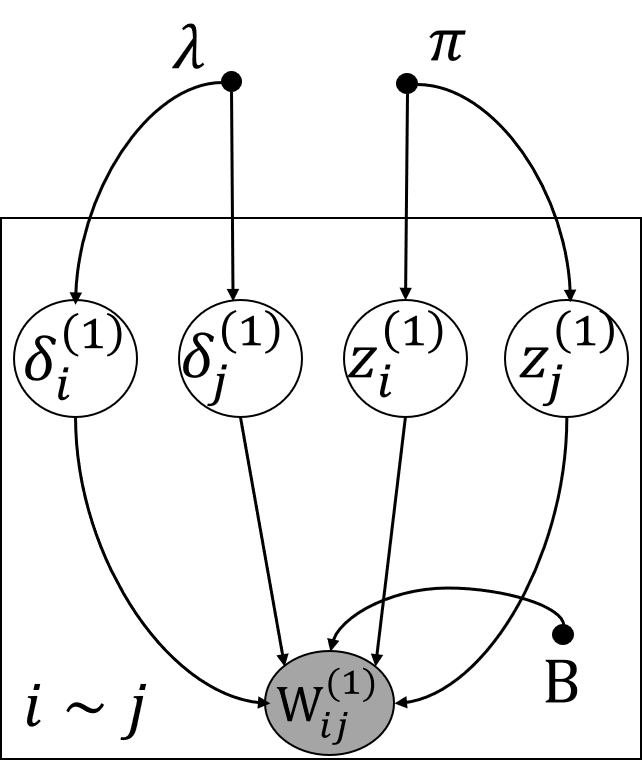
\includegraphics[width=.26\textwidth]{figures/chap05/graph1.png}
    }
    \subfigure[网络快照$t >1$的图模型]{
        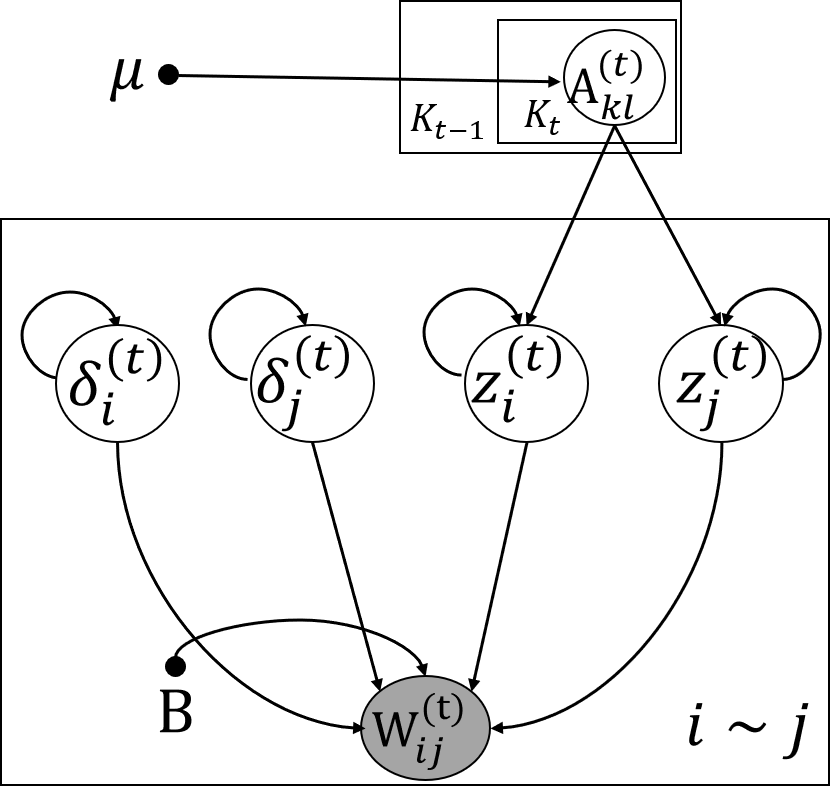
\includegraphics[width=.32\textwidth]{figures/chap05/graph2.png}
    }
    \caption{本文提出的GEABS方法的图模型}
    \label{fig:graphmodel}
    %\vspace{-0.1in}
\end{figure}


该过程类似于随机块模型(SBM)的生成,$\pi \in (0,1)^{K^{(1)}}$ 是多项分布的参数向量,其中$\sum_k \pi_k =1$,该分布用于控制节点归属不同社团的概率。$B \in (0,1)^{K^{(1)} \times K^{(1)}}$ 是分属不同社团间的节点的连边概率,即在各自社团中的任意两个节点之间存在边的概率。
随后,从具有 $\pi$ 的多项分布中为每个节点采样潜在变量 $Z_i^{(1)}$作为节点$i$的社团划分。最后,对于每对节点 $i \ne j$,$W^{(1)}_{ij}$ 从 $Bernoulli(B_{z_i^{(1)} z_j^{(1)}})$ 中采样以获得连边。

然而经典随机块模型并未建模节点异质性,这意味着同一社团内的节点在与其他社团中的节点的交互过程是等价的。为了建模网络中节点的异质性,本章为节点$i$设计了流行度参数 $\delta^{(1)}_i$,本章将其视为可学习参数而不是确定值(例如节点的度),这使得该参数能够更好得建模节点的异质性(见前文数据挖掘部分\ref{chap:3}),引入节点流行度参数后的节点连边概率即为 $W^{(1)}_{ij} \sim Bernoulli\left(B_{z_i^{(1)} z_j^{(1)}}^{1+\delta_i^{(1)} + \delta_j^{(1)}}\right)$。这种建模方式可以提升模型对真实世界网络的建模能力,避免了同一社团内节点的同质性表现。后续实验也证明了,该设计可以捕获真实世界网络中的幂律分布,比经典随机块模型和度修正的随机块模型更具有优势。

\subsubsection{$G^{(t>1)}$时刻的生成过程}

对于网络快照$t > 2$,本节以$t-1$到$t$为例进行介绍。首先,流行参数的生成$\delta_i^{(t)}$依赖于$\delta_i^{(t-1)}$,本方法采用指数分布来刻画这种关系,即$\delta_i^{(t)} \sim Exp(\delta_i^{t-1})$。对于社团演化,本方法定义了社团转移矩阵$A^{(t)}$来刻画社团层面的演化,$A^{(t)}_{kl}$ 表示一个节点从快照$t-1$时刻的社团$k$转移到$t$时刻的社团$l$的概率,且 $\sum_{l=1}^{K^{(t)}}A^{(t)}_{kl}$,其中$k =\{1, \cdots, K^{(t-1)}\}$。对于网络快照$t$的隐变量生成,如图~\ref{fig:graphmodel} (b) 所示,依据\textbf{算法~\ref{gent2}}实现动态网络的生成与演化建模。

其中,概率转移矩阵$A^{(t)}$表示社团层面的演化,该矩阵的变化可以揭示不同的社团行为。考虑到社团行为与社团异常之间的关系,本章将在后续基于参数$A^{(t)}$来识别社团异常行为。通过该生成过程,GEABS可以在一个统一的框架下建模动态网络的节点流行度、社团结构及其演化。结合后续的异常检测指标定义,GEABS还可以对多尺度的动态网络异常演化行为进行识别。

这里,本章给出关于GEABS模型的详细补充说明:
\begin{itemize}
    \item 对于模型中的分布选择,例如狄利克雷分布、Beta分布和多项分布及其先验分布,可以考虑共轭分布和网络特性进行灵活选择。
    \item  对于参数$\lambda$、$\pi$ 和 $\mu$,GEABS可以使用一般和共轭分布来进行后验推断,无需额外的超参数进行描述。
    \item  对于动态网络中的快照节点数量差异,可以在快照之间添加差异节点或取连续快照的节点并集来生成观测结构。
    \item  本章用伯努利分布生成$W^{(t)}_{ij}$,这仅适用于无权网络。对于有权网络,可以改用泊松或指数分布对节点的连边情况及权重进行生成。
\end{itemize}

% For snapshot $t > 2$, we should analyze the evolution across the snapshots from $t-1$ to $t$. First, the popular parameter $\delta_i^{(t)}$ is depend on $\delta_i^{(t-1)}$, we take the Exponential distribution to describe the relationship, i.e. $\delta_i^{(t)} \sim Exp(\delta_i^{t-1})$. For the community variable, we define a probability transition matrix $A^{(t)}$ to describe the community level evolution, $A^{(t)}_{kl}$ is denoted as the probability of one node transiting from  community $k$ at snapshot $t-1$ to community $l$ at $t$ and $\sum_{l=1}^{K^{(t)}}A^{(t)}_{kl}$, for $k =1, \cdots, K^{(t-1)}$. With the latent variables for network snapshot $t$, as in Fig.~\ref{fig:graphmodel} (b), we can generate the observed structure with \textbf{Algorithm~\ref{gent2}}.

% Here, the probability transition matrix $A^{(t)}$ represents the community level evolution, it could reveal the different behaviors. Considering the relationship between community behavior and anomaly, we will denote its abnormal behavior based on $A^{(t)}$ later. With this generative process, we can model the varying of dynamic networks with node popularity, community structure and its evolution under a unified framework. Then, our GEABS model can reveal the temporal behaviors and the anomaly on different scales.




% Here, we give some supplementary remarks about the GEABS model for details.
% %% 补充说明:W相似矩阵,社团变化,节点变化,超参数说明,分布选择
% \begin{itemize}
%     \item The choice of these distributions, e.g., Dirichlet, Beta and multinomial, should satisfy the conjugate distribution and network properties as much as possible.
%     \item  Regarding the parameters $\lambda$, $\pi$ and $\mu$, we can use general and conjugate distributions to generate them without additional hyperparameters.
%     \item Changing the number of nodes in the dynamic network, we can add the differential nodes across the snapshots or take the union of nodes of consecutive snapshots for generating the observed structure.
%     \item We only generate $W^{(t)}_{ij}$ with Bernoulli distribution, which is only suitable for binary networks.
%     For weighted or real-valued networks, Poisson or exponential distributions can be used instead.
% \end{itemize}

\begin{algorithm}[H]
\caption{$t \ge 2$的网络快照的生成过程}\label{gent2}
\begin{algorithmic}[1]
\STATE \textbf{输入:} 先验参数$\mu$, 节点流行度参数$\delta^{(t-1)}$ 社团划分$Z^{(t-1)}$ \\
\STATE \textbf{输出:} 网络快照 $W^{(t)}$
\STATE 超参数初始化
\STATE ~~~~采样 $\mu \sim Dirichlet (1)$ 
\STATE ~~~~采样 $B \sim Beta(1,1)$
\STATE 采样 $A^{(t)}$
\FOR{$k=1, 2, \cdots, K^{(t-1)}$}
\STATE $A^{(t)}_{k\cdot} \sim Dirichlet(\mu)$
\ENDFOR
\STATE 采样 $Z^{(t)}$ 和 $\delta^{(t)}$
\FOR{$i=1, 2, \cdots, N$}
\STATE 采样 $\delta^{(t)}_i \sim Exp(\delta^{(t-1)}_i)$
\STATE 采样 $Z^{(t)}_i \sim Multi(A^{(t)}_{Z_i^{t-1}})$
\ENDFOR
\STATE 生成$G^{(t)}的邻接矩阵$
\FOR{$i=1, 2, \cdots, N-1, j=2, \cdots, N$}
%\FOR{$i=1, 2, \cdots, N-1$}
%\FOR{$j=2, \cdots, N$}
\STATE 采样 $W^{(t)}_{ij} \sim Bernoulli(B_{z_i^{(t)} z_j^{(t)}}^{1+\delta_i^{(t)} + \delta_j^{(t)}})$
%\ENDFOR
\ENDFOR
\end{algorithmic}
\end{algorithm}

\subsection{模型的参数近似后验推断}



GEABS模型有两种形式化方法,分别为在线方法和离线方法。前者只关注快照$t$及其之前的网络数据,后者则会同时考虑动态网络的所有快照。本节只给出离线的形式化表示(离线的形式化表示推断更加全面)。

在快照$t=1$,基于图模型及其生成过程,观测变量$W^{(1)}$和隐变量 $Z^{(1)}$及$\delta^{(t)}$的联合概率分布如下:
\begin{align}
O_1 = & Pr(W^{(1)}, Z^{(1)}, \delta^{(1)} |\pi, \lambda, B) \nonumber\\
= & Pr(W^{(1)}|Z^{(1)},B,\delta^{(1)})  Pr(\delta^{(1)}|\lambda) Pr(Z^{(1)}|\pi),
\label{eq:O1}
\end{align}
其中 $Pr(Z^{(1)} | \pi)$ 是第一个快照$t=1$中的社团划分的概率分布,$Pr(\delta^{(1)} | \lambda)$ 是初始节点流行度的概率分布。它们可以表示为:
\begin{align}
Pr (Z^{(1)}|\pi) &= \prod_{i=1}^{N} Pr(z_i^{(1)}|\pi) = \prod_{i=1}^{N} \pi_{z_i^{(1)}}, 
\label{eq:O6}\\
Pr (\delta^{(1)}|\lambda)  &= \prod_{i=1}^{N} Pr(\delta_i^{(1)}|\lambda)
 = \prod_{i=1}^{N} \lambda e^{-\lambda \delta_i^{(1)}}. 
\label{eq:O7}
\end{align}

类似地,在快照$t$时可以写出如下公式:
\begin{align}
O_t = & Pr(W^{(t)}, Z^{(t)}, \delta^{(t)}, A^{(t)} |\mu, Z^{(t-1)}, \delta^{(t-1)}, B) \nonumber\\
= & Pr(W^{(t)}|Z^{(t)},B,\delta^{(t)})  Pr(\delta^{(t)}|\delta^{(t-1)}) \nonumber\\ 
&\qquad Pr(Z^{(t)}|Z^{(t-1)}, A^{(t)}) Pr(A^{(t)} | \mu).
\label{eq:O2}
\end{align}

% where $Pr(Z^{(1)} | \pi)$ is the probability of community assignment in first snapshot $t-1$, and $Pr(\delta^{(1)} | \lambda)$ is the probability distribution of initial popularity. They can be calculated as:
% \begin{align}
% Pr (Z^{(1)}|\pi) &= \prod_{i=1}^{N} Pr(z_i^{(1)}|\pi) = \prod_{i=1}^{N} \pi_{z_i^{(1)}}, 
% \label{eq:O6}\\
% Pr (\delta^{(1)}|\lambda)  &= \prod_{i=1}^{N} Pr(\delta_i^{(1)}|\lambda)
%  = \prod_{i=1}^{N} \lambda e^{-\lambda \delta_i^{(1)}}. 
% \label{eq:O7}
% \end{align}


% Similarity, we can write it at snapshot $t$ as follows:%Eq.~\ref{eq:O2}
% \begin{align}
% O_t = & Pr(W^{(t)}, Z^{(t)}, \delta^{(t)}, A^{(t)} |\mu, Z^{(t-1)}, \delta^{(t-1)}, B) \nonumber\\
% = & Pr(W^{(t)}|Z^{(t)},B,\delta^{(t)})  Pr(\delta^{(t)}|\delta^{(t-1)}) \nonumber\\ 
% &\qquad Pr(Z^{(t)}|Z^{(t-1)}, A^{(t)}) Pr(A^{(t)} | \mu).
% \label{eq:O2}
% \end{align}


% In the case of the probability distribution proposed above, the detailed formalization is as in Eqs.~\ref{eq:O3}-\ref{eq:O5}.
% where, with the probability distribution proposed above, detailed formalization are as Eqs.~\ref{eq:O3}-\ref{eq:O7}.

% \begin{equation}
% \begin{split}
% Pr&(W,Z,\delta|\pi,B,A,\lambda) \\
% =    &   \prod_{t=1}^{T} Pr(W^{(t)}|Z^{(t)},B,\delta^{(t)}) \prod_{t=2}^{T} Pr(Z^{(t)}|Z^{(t-1)},A^{(t)})   \\
% & Pr(Z^{(1)}|\pi) Pr(\delta^{(1)}|\lambda) \prod_{t=2}^{T} Pr(\delta^{(t)}|\delta^{(t-1)}) \prod_2^{T} Pr(A^{(t)} | \mu)\\
% \end{split}
% \end{equation}
% Where the connection probability $Pr(W^{(t)}|Z^{(t)},B,\delta^{(t)})$ is
% \begin{align}
%    &Pr  (W^{(t)}|Z^{(t)},B,\delta^{(t)}) = \prod_{i \sim j} Pr(W^{(t)}_{ij}|z^{(t)}_i ,z^{(t)}_j, B, \delta^{(t)}_i, \delta^{(t)}_j )   \nonumber  \\
% & = \prod_{w_{ij}^{(t)}=1} B_{z_i^{(t)} z_j^{(t)}}^{1+\delta_i^{(t)}+\delta_j^{(t)}}  \prod_{w_{ij}^{(t)}=0} (1-B_{z_i^{(t)} z_j^{(t)}}^{1+\delta_i^{(t)}+\delta_j^{(t)}}),     
% \label{eq:O3}\\
% &Pr(Z^{(t)}|Z^{(t-1)},A) = \prod_{i=1}^{N} Pr(z_i^{(t)} | z_i^{(t-1)},A )= \prod_{i=1}^{N} A_{z_i^{(t-1)} z_i^{(t)}},  
% \label{eq:O4}\\
% &Pr (\delta^{(t)}|\delta^{(t-1)})  = \prod_{i=1}^{N} Pr(\delta_i^{(t)}|\delta_i^{(t-1)}) = \prod_{i=1}^{N} \delta_i^{(t-1)} e^{-\delta_i^{(t-1)} \delta^{(t)}},
% \label{eq:O5}
% \end{align}
% where $Pr(W^{(t)}|Z^{(t)},B,\delta^{(t)})$ is the conditional probability of $W^{(t)}$, $Pr(\delta^{(t)}|\delta^{(t-1)})$ is the varying probability of node popularity, and $Pr(Z^{(t)}|Z^{(t-1)},A^{(t)})$ is the transition probability across the snapshots for $t=2, \cdots, T$.

% We choose the exponential distribution to model the varying of $\delta^{(t)}$, i.e., $\delta_i^{(t)} \sim Exp(\delta_i^{(t-1)})$, it is easy to know that $E(\delta_i^{(t)}) = \frac{1}{\delta_i^{(t-1)}}$. With this, if the node popularity has not changed significantly, $\delta_i^{(t)} \approx 1$. However, if it has a significant change and fits the network snapshot well, this means it may be a change point. Besides, with the Dirichlet distribution for the probability transition matrix $A^{(t)}$, the joint probability distribution of the model is given as:
% \begin{align}
% O = & Pr(W, Z,\delta, A|\pi, \lambda, \mu, B) = Q_1 \prod_{t=2}^{T} O_t \nonumber \\
% =  & \prod_{t=1}^{T} \Big[\prod_{w_{ij}^{(t)}=1} b_{z_i^{(t)} z_j^{(t)}}^{1+\delta_i^{(t)}+\delta_j^{(t)}}  \prod_{w_{ij}^{(t)}=0} (1-b_{z_i^{(t)} z_j^{(t)}}^{1+\delta_i^{(t)}+\delta_j^{(t)}})\Big]  \nonumber  \\
% & \prod_{t=2}^{T} \prod_{i=1}^{n} A_{z_i^{(t-1)} z_i^{(t)}}  \prod_{t=2}^{T} \prod_{k} \frac{\Gamma (\sum_l \mu_{kl})}{\prod_l \Gamma (\mu_{kl})} \prod_l {A^{(t)}_{kl}}^{\mu_{kl} - 1} \nonumber\\
%  &\prod_{t=2}^{T} \prod_{i=1}^{N} \delta_i^{(t-1)} e^{-\delta_i^{(t-1)} \delta_i^{(t)}} \prod_{i=1}^{N} \pi_{z_i^{(1)}}  \prod_{i=1}^{N} \lambda e^{-\lambda \delta_i^{(1)}}. 
% \label{eq:O8}
% \end{align}

% \subsection{Evolutionary Anomaly Detection}
% With our GEABS model, if we have learned the variable parameters $\delta$, $Z$ and $A$, which can characterize the node level activity and popularity, community structure and its evolutionary activity, respectively. To capture the different levels of anomaly, we further define the three levels of anomaly detection.

% At the \textbf{network level}, it also is called a change point in dynamic networks, its essence is to calculate the difference between two snapshots.
% By combining the node level popularity $\delta$ and the community level transition parameter $A$ and community structure $Z$, the network level anomaly value at snapshot $t$ is defined as follows:%Eq.~\ref{eq:O9}.
% \begin{equation}
%     E_{nl}^{(t)} = \sum_{i, k} e^{A_{z_i^{(t)} k}^t  (1-I(z_i^{(t)},z_i^{(t-1)}))} \| \delta_i^{(t)} - \delta_i^{(t-1)} \|_2^2,
% \label{eq:O9}
% \end{equation}
% where the node popularity, community structure and transition probability are integrated across the snapshots. If the node $V_i$ belongs to the same community, the anomaly value only depends on the varying of node popularity, otherwise, this value is corrected by the transition probability in $A^{(t)}$. Furthermore, for the set $\mathcal{t} = \{t : |f(G^{(t-1)}) -f(G^{(t)})| > \epsilon  \} $, where the function $f = E_{nl}^{(t)}$.
% Besides, the choice of $\epsilon$ is usually replaced by the Top-K values.

% At the \textbf{community level}, if community structure $Z^{(t-1)}$ and $Z^{(t)}$ have a significant difference, it means there are community events, e.g., community growth and contraction, merge and split. In this paper, we analyze the anomaly behaviors based on the transition probability matrix $A^{(t)}$. Considering that community detection is an unsupervised problem, matching communities on different snapshots is also an interesting issue, with basic mapping way, some important community behaviors, such as merge and split, growth and contraction can be captured with our $A^{(t)}$.

% At the \textbf{node level}, based on the community membership $Z = \{ Z^{(1)}, Z^{(2)}, \cdots, Z^{(T)} \}$, if one node changes community affiliation frequently, it should be abnormal in the dynamic network. So we denote the anomaly value of nodes based on the community structure and as Eq.~\ref{eq:networkanomaly}.
% \begin{equation}
%     {E_{cl}}_{(i)} = \frac{\sum_t^T \delta_i^{(t)}}{T} H(Z_i^{(1):(T)}),
% \label{eq:networkanomaly}
% \end{equation}
% where $H(Z_i^{(1):(T)})$ is the Entropy measure, while $Z_i^{(1):(T)}$ is the total community memberships node $i$ belonging to from $t=1$ to $t=T$. Therefore,  $Z_i^{(1):(T)}$ is a vector representing the whole community membership of node $V_i$.


% Just as described before, we believe that if an important node switch its community membership, it will seriously affect the behavior of its community, and then affect the evolution of the entire network. So the node level anomaly parameter is defined  as:

% \begin{equation}
% \begin{split}
%     E_{nl}^{(t)} = \delta_i^{(t)} Entropy(z_i^{(t)}, z_i^{(t-1)})
% \end{split}
% \label{eq:networkanomaly}
% \end{equation}

% 其中,基于上述概率分布,详细的形式化如 Eqs.~\ref{eq:O3}-\ref{eq:O7} 所示。
因此,该模型的联合概率分布可初步写为:
\begin{equation}
\begin{split}
Pr&(W,Z,\delta|\pi,B,A,\lambda) \\
=    &   \prod_{t=1}^{T} Pr(W^{(t)}|Z^{(t)},B,\delta^{(t)}) \prod_{t=2}^{T} Pr(Z^{(t)}|Z^{(t-1)},A^{(t)})   \\
& Pr(Z^{(1)}|\pi) Pr(\delta^{(1)}|\lambda) \prod_{t=2}^{T} Pr(\delta^{(t)}|\delta^{(t-1)}) \prod_{t=2}^{T} Pr(A^{(t)} | \mu).\\
\label{eq:03}
\end{split}
\end{equation}
在上述概率分布的情况下,动态网络的观测值及隐变量的详细形式化如 公式~\ref{eq:031}-\ref{eq:05} 所示。其中,连边概率$Pr(W^{(t)}|Z^{(t)},B,\delta^{(t)})$的更新公式、社团划分矩阵的更新公式$Pr(Z^{(t)}|Z^{(t-1)},A^{(t)})$以及节点流行度参数的更新公式$Pr(\delta^{(t)}|\delta^{(t-1)})$ 分别为:
\begin{align}
   &Pr  (W^{(t)}|Z^{(t)},B,\delta^{(t)}) = \prod_{i \sim j} Pr(W^{(t)}_{ij}|z^{(t)}_i ,z^{(t)}_j, B, \delta^{(t)}_i, \delta^{(t)}_j )   \nonumber  \\
& = \prod_{w_{ij}^{(t)}=1} B_{z_i^{(t)} z_j^{(t)}}^{1+\delta_i^{(t)}+\delta_j^{(t)}}  \prod_{w_{ij}^{(t)}=0} (1-B_{z_i^{(t)} z_j^{(t)}}^{1+\delta_i^{(t)}+\delta_j^{(t)}}),     
\label{eq:031}\\
&Pr(Z^{(t)}|Z^{(t-1)},A) = \prod_{i=1}^{N} Pr(z_i^{(t)} | z_i^{(t-1)},A )= \prod_{i=1}^{N} A_{z_i^{(t-1)} z_i^{(t)}},  
\label{eq:04}\\
&Pr (\delta^{(t)}|\delta^{(t-1)})  = \prod_{i=1}^{N} Pr(\delta_i^{(t)}|\delta_i^{(t-1)}) = \prod_{i=1}^{N} \delta_i^{(t-1)} e^{-\delta_i^{(t-1)} \delta^{(t)}},
\label{eq:05}
\end{align}
% 其中 $Pr(W^{(t)}|Z^{(t)},B,\delta^{(t)})$ 是 $W^{(t)}$ 的条件概率,$Pr(\delta^{(t)}|\delta^{(t-1)})$ 是节点流行度的更新概率,$Pr(Z^{(t)}|Z^{(t-1)},A^{(t)})$,对于 $t=2, \cdots, T$。

值得注意的是,GEABS选择指数分布来建模$\delta^{(t)}$的变化,即 $\delta_i^{(t)} \sim Exp(\delta_i^{(t-1)})$,易知$t$时刻的节点流行度的期望$E(\delta_i^{(t)}) = \frac{1}{\delta_i^{(t-1)}}$。
% 如果节点流行度没有显著变化,则$\delta_i^{(t)} \approx 1$。然而,如果它有显著变化并且网络快照,这意味着它可能是一个变化点。
此外,对于概率转移矩阵$A^{(t)}$,使用狄利克雷分布进行刻画。
将上述分布带入,得出模型的联合概率分布如下:
\begin{align}
O = & Pr(W, Z,\delta, A|\pi, \lambda, \mu, B) = Q_1 \prod_{t=2}^{T} O_t \nonumber \\
=  & \prod_{t=1}^{T} \Big[\prod_{w_{ij}^{(t)}=1} b_{z_i^{(t)} z_j^{(t)}}^{1+\delta_i^{(t)}+\delta_j^{(t)}}  \prod_{w_{ij}^{(t)}=0} (1-b_{z_i^{(t)} z_j^{(t)}}^{1+\delta_i^{(t)}+\delta_j^{(t)}})\Big]  \nonumber  \\
& \prod_{t=2}^{T} \prod_{i=1}^{n} A_{z_i^{(t-1)} z_i^{(t)}}  \prod_{t=2}^{T} \prod_{k} \frac{\Gamma (\sum_l \mu_{kl})}{\prod_l \Gamma (\mu_{kl})} \prod_l {A^{(t)}_{kl}}^{\mu_{kl} - 1} \nonumber\\
 &\prod_{t=2}^{T} \prod_{i=1}^{N} \delta_i^{(t-1)} e^{-\delta_i^{(t-1)} \delta_i^{(t)}} \prod_{i=1}^{N} \pi_{z_i^{(1)}}  \prod_{i=1}^{N} \lambda e^{-\lambda \delta_i^{(1)}}. 
\label{eq:O8}
\end{align}

\subsection{动态网络层次演化异常检测定义}
本章的GEABS模型所建模的变量 $\delta$、$Z$ 和 $A$分别可以表示节点层次的流行度、社团级别的结构及其演化。为了捕捉不同层次的异常,本章进一步定义了三层次的异常指标以刻画动态网络的层次异常。

在\textbf{网络层次},其异常也被称为动态网络的变更点,其本质是严重违背动态网络平滑性假设的网络快照,此类快照的识别能够帮助更好地对动态网络进行建模及挖掘。考虑到网络快照层次的变化往往受节点及社团的影响,即当网络中存在影响力过大的节点的剧烈变化及社团的剧烈变化时,会导致网络出现变更点。因此网络层次的异常本文通过结合节点流行度$\delta$和社团层次的转移参数$A$以及社团结构$Z$来定义快照$t$时的网络层次异常值:
\begin{equation}
    E_{nl}^{(t)} = \sum_{i, k} e^{A_{z_i^{(t)} k}^t  (1-I(z_i^{(t)},z_i^{(t-1)}))} \| \delta_i^{(t)} - \delta_i^{(t-1)} \|_2^2,
\label{eq:O9}
\end{equation}

如果节点$V_i$在相邻快照属于同一社团,则网络级别异常值仅依赖于节点流行度的变化,否则,该值由$A^{(t)}$中的社团转移概率进行校正,这可以保证该值在真实世界符合重尾分布的动态网络中能够捕获所累积的变化。为了识别网络异常,本章将异常快照的集合定义为$\mathcal{t} = \{t : |f(G^{(t-1)}) -f(G^{(t)})| > \epsilon  \}$,其中函数$f = E_{nl}^{(t)}$。而$\epsilon$的选择通常以动态网络快照级别异常值的$Top-K$值替代进行替代,即通过对快照异常值进行排序,以前$K$个为准。

在 \textbf{社团层次},如果动态网络社团结构$Z^{(t-1)}$和$Z^{(t)}$ 有显著差异,这意味着相邻快照中存在社团级别的事件,例如社团增长和收缩、合并和分裂等。本章基于转移概率矩阵$A^{(t)}$分析社团级别的异常行为。考虑到社团检测是一个无监督问题,匹配不同快照上的社团也是一个有趣的问题,因此本章的社团级别异常主要以$A^{(t)}$为异常参数,并通过设计动态快照社团匹配来进行启发式的识别,这可以更好地捕捉重要的社团行为,例如合并和分裂、增长和收缩等(详见实验\ref{community anomaly})。

在 \textbf{节点层次},基于社团划分关系 $Z = \{ Z^{(1)}, Z^{(2)}, \cdots, Z^{(T)} \}$进行识别,本文认为如果一个节点频繁改变社团归属,它在动态网络中应被视为异常演化模式。因此,本章基于社团划分的变化程度表示节点的异常值,如 Eq.~\ref{eq:networkanomaly} 所示。
\begin{equation}
    {E_{cl}}_{(i)} = \frac{\sum_t^T \delta_i^{(t)}}{T} H(Z_i^{(1):(T)}),
\label{eq:networkanomaly}
\end{equation}
其中 $H(Z_i^{(1):(T)})$ 为熵,而$Z_i^{(1):(T)}$是节点$v_i$ 从 $t=1$到$t=T$所属的所有社团划分的关系。故$Z_i^{(1):(T)}$表示节点$v_i$在整个动态网络快照中的社团归属向量。

% 如前所述,本章认为如果一个重要节点改变其社团成员关系,它将严重影响其社团的行为,进而影响整个网络的演化。因此,节点层次的异常参数定义为:
% \begin{equation}
% \begin{split}
%     E_{nl}^{(t)} = \delta_i^{(t)} Entropy(z_i^{(t)}, z_i^{(t-1)})
% \end{split}
% \label{eq:networkanomaly}
% \end{equation}

\section{融合节点流行度的动态随机块模型的推断及参数求解}
\label{sec4:inference}
为了优化公式~\ref{eq:O8}的联合分布,需要计算给定观测变量和超参数的后验函数,可以写成如下形式:
\begin{equation}
Pr(Z,\delta, A, \pi, \lambda, B | W, \mu) =
\frac{Pr(W, Z,\delta, A, \pi, \lambda, \mu, B)}{Pr( W, \mu)}.
\label{eq:OA1}
\end{equation}
然而,直接计算公式~\ref{eq:OA1}是不可行的,因此本文通过变分推断,引入一个新的变分分布$q$来近似原参数的后验分布,其定义如下:
\begin{equation}
\begin{split}
q(\phi,\bar{\delta}, \tilde{\mu}) = \prod_t \Big[ \prod_i q(\phi_i^{(t)}) \prod_i q(\bar{\delta}_i^{(t)}) \prod_k \prod_l q(\tilde{\mu}_{kl}^{(t)}) \Big],
\end{split}
\label{qfunc}
\end{equation}

其中,$\phi$、$\bar{\delta}$ 和 $\tilde{\mu}$ 是公式~\ref{eq:O8} 联合分布中 $Z$、$\delta$ 和 $A$ 的变分参数。  
具体来说:$z_i^t \sim Multi(\phi_i^{(t)})$,表示节点 $i$ 在时间 $t$ 的社区分配 $z_i^t$ 服从以 $\phi_i^{(t)}$ 为参数的多项分布;$\delta_i^{(t)} \sim \mathbf{1}(\bar{\delta_i^{(t)}})$,表示节点 $i$ 在时间 $t$ 的活跃状态 $\delta_i^{(t)}$ 服从以 $\bar{\delta_i^{(t)}}$ 为参数的指示分布;$A_{kl}^{(t)} \sim Dirichlet(\tilde{\mu}_{kl}^{(t)})$,表示社区 $k$ 到社区 $l$ 在时间 $t$ 的转移概率 $A_{kl}^{(t)}$ 服从以$\tilde{\mu}_{kl}^{(t)}$ 为参数的狄利克雷分布。而$q(\phi_i^{(t)})$表示$z_i^{(t)}$ 的近似后验分布;$q(\delta_i^{(t)})$表示$\delta_i^{(t)}$ 的近似后验分布;$\tilde{\mu}_{kl}^{(t)}$则表示$A_{kl}^{(t)}$ 的近似后验分布。下面将具体介绍变分EM步的对应参数更新公式的推断过程。

通过变分推断以及公式~\ref{qfunc}中的定义,利用Jensens不等式,其对数似然的下界可以表示为公式~\ref{qfunc1},并且满足$\log Pr(W) = KL(q \| p) + \mathscr{L}(q)$。  
\begin{equation}
\log Pr(W)\ge E_q(\log Pr(W, Z,\delta, A) ) + H(q),
\label{qfunc1}
\end{equation}
忽略对数似然中的无关参数,$H(q)$表示变分分布的熵。$q$和$p$分别是近似后验分布和真实后验分布,$\mathscr{L}(q)$是变分推断的证据下界(即变分下界ELBO)。根据上式可以看出,最小化$KL(q \| p)$可以转化为最大化变分下界$\mathscr{L}(q)$。  
完整的模型ELBO可以表示为~\ref{ELBO}。
\begin{align}
 \mathscr{L} & (Z,\bar{\delta},\tilde{\mu};\pi,B,\lambda,\mu) \nonumber \\
& = \sum_{t=1}^T \sum_{w_{ij}^{(t)}=1} (1+\bar{\delta}_i^{(t)}+\bar{\delta}_j^{(t)}) \sum_k \sum_l \phi_{ik}^{(t)}\phi_{jl}^{(t)} \log B_{kl} \nonumber\\
& -\sum_{t=1}^T \sum_{w_{ij}^{(t)}=0} \sum_k \sum_l \phi_{ik}^{(t)}\phi_{jl}^{(t)}  B_{kl}^{1+\bar{\delta}_i^{(t)}+\bar{\delta}_j^{(t)}} \nonumber\\
& +\sum_{t=2}^T \sum_i \sum_k \sum_l \phi_{ik}^{(t-1)}\phi_{il}^{(t)} [\psi(\tilde{\mu}_{kl}^{(t)}) - \psi(\sum_l \tilde{\mu}_{kl}^{(t)})]  \nonumber\\
& +\sum_i \sum_k \phi_{ik}^{(1)} \log \pi_k +  N\log \lambda -\lambda \sum_i \bar{\delta}_i^{(1)}  \nonumber \\
& +\sum_{t=2}^T \sum_k \sum_l(\mu_{kl} - 1) \Big[\psi(\tilde{\mu}_{kl}^{(t)}) - \psi(\sum_l \tilde{\mu}_{kl}^{(t)})\Big]  \nonumber\\
& + \sum_{t=2}^{T} \sum_{i=1}^N \big[\log \bar{\delta}_i^{t-1} - \bar{\delta}_i^{t-1} \bar{\delta}_i^{t}\big] -E_q \log q.
\label{ELBO}
\end{align}

\subsection{隐变量更新公式推断}

在GEABS模型中,快照$t=1$的隐变量依赖于快照$t=2$的隐变量,而快照$T$的变量则受$T-1$的约束。对于快照$t=2, \cdots, T-1$的变量,其推断受到前后两个快照的组合影响。参数及隐变量的更新公式推断详细内容见附录命题~\ref{GEABS:inference},这里给出更新公式。
\subsubsection{$t=1$时的隐变量更新公式}
当$t=1$时,$\phi_{ik}^{(1)}$的更新规则为:
\begin{equation}
\begin{split}
\phi _{ik}^{(1)} & \propto \pi_k \exp\{ \sum_{w_{ij}^{(1)}=1} (1+\bar{\delta}_i^{(1)}+\bar{\delta}_j^{(1)}) \sum_l \phi_{jl}^{(1)} \log B_{kl} \\
& -\sum_{w_{ij}^{(1)}=0} \sum_l \phi_{jl}^{(1)}  b_{kl}^{1+\bar{\delta}_i^{(1)}+\bar{\delta}_j^{(1)}} \\
& + \sum_l \phi_{il}^{(2)}[\psi(\tilde{\mu}_{kl}^{(2)}) - \psi(\sum_l \tilde{\mu}_{kl}^{(2)})] \},
\end{split}
\end{equation}

$\bar{\delta}_i^{(1)}$的梯度为:
\begin{equation}
\begin{split}
\frac{\partial \mathscr{O}(\bar{\delta}_i^{(1)})}{\partial \bar{\delta}_i^{(1)}} & =\sum_{w_{ij}^{(1)}=1} \sum_k \sum_l \phi_{ik}^{(1)}\phi_{jl}^{(1)} \log B_{kl} \\
& -\sum_{w_{ij}^{(1)}=0} \sum_k \sum_l \phi_{ik}^{(1)}\phi_{jl}^{(1)}  B_{kl}^{1+\bar{\delta}_i^{(1)}+\bar{\delta}_j^{(1)}} \log B_{kl} \\
& -\lambda - \bar{\delta}_i^{(2)} + \frac{1}{\bar{\delta}_i^{(1)}},
\end{split}
\label{eq:delta1}
\end{equation}

\subsubsection{$1<t<T$时的隐变量更新公式}
$\phi_{ik}^{(t)}$、$\tilde{\mu}_{kl}^t$、$\frac{\partial \mathscr{L}_t}{\partial \bar{\delta}_i^{(t)}}$的更新规则如公式~\ref{eq:phit} ~\ref{eq:A}和~\ref{eq:deltat} 所示:
   \begin{equation}
   \begin{split}
   &\phi_{ik}^{(t)} \propto \exp\bigg\{ \sum_{w_{ij}^{(t)}=1} (1+\bar{\delta}_i^{(t)}+\bar{\delta}_j^{(t)}) \sum_l \phi_{jl}^{(t)} \log B_{kl} \\
   & -\sum_{w_{ij}^{(t)}=0} \sum_l \phi_{jl}^{(t)}  B_{kl}^{1+\bar{\delta}_i^{(t)}+\bar{\delta}_j^{(t)}}  \\
  & +\sum_k \phi_{ik}^{(t-1)} \Big[\psi(\tilde{\mu}_{kl}^{(t)}) - \psi(\sum_l \tilde{\mu}_{kl}^{(t)})\Big] \\
   &+ \sum_l \phi_{il}^{(t+1)} \Big[\psi(\tilde{\mu}_{kl}^{(t+1)}) - \psi(\sum_l \tilde{\mu}_{kl}^{(t+1)})\Big] \bigg\},
   \label{eq:phit}
   \end{split}
   \end{equation}

   \begin{equation}
   \tilde{\mu}_{kl}^t = \sum_i \phi_{il}^{(t-1)} \phi_{ik}^{(t)} + \mu_{kl},
   \label{eq:A}
   \end{equation}


\begin{align}
\frac{\partial \mathscr{L}_t}{\partial \bar{\delta}_i^{(t)}} & =\sum_{w_{ij}^{(t)}=1} \sum_k \sum_l \phi_{ik}^{(t)}\phi_{jl}^{(t)} \log B_{kl}  \nonumber\\
& -\sum_{w_{ij}^{(t)}=0} \sum_k \sum_l \phi_{ik}^{(t)}\phi_{jl}^{(t)}  B_{kl}^{1+\bar{\delta}_i^{(t)}+\bar{\delta}_j^{(t)}} \log B_{kl} \nonumber\\
& -\bar{\delta}_i^{(t-1)} - \bar{\delta}_i^{(t+1)} - \log \bar{\delta}_i^{(t)} - 1.
\label{eq:deltat}
\end{align}



\subsubsection{$t=T$时的隐变量更新公式}

$\phi_i^{(t)}$的更新公式为:


\begin{equation}
\begin{split}
\phi_{ik}^{(T)} & \propto \exp\{ \sum_{w_{ij}^{(T)}=1} (1+\bar{\delta}_i^{(T)}+\bar{\delta}_j^{(T)}) \sum_l \phi_{jl}^{(T)} \log B_{kl} \\
& -\sum_{w_{ij}^{(T)}=0} \sum_l \phi_{jl}^{(T)}  b_{kl}^{1+\bar{\delta}_i^{(T)}+\bar{\delta}_j^{(T)}}  \\
& + \sum_l \phi_{il}^{(T-1)} [\psi(\tilde{\mu}_{kl}^{(T)}) - \psi(\sum_l \tilde{\mu}_{kl}^{(T)})] \},
\end{split}
\label{eq:phiT}
\end{equation}

$\bar{\delta}_i^{(T)}$的更新公式如下:



\begin{equation}
\begin{split}
& \frac{\partial \mathscr{O}(\bar{\delta}_i^{(T)})}{\partial \bar{\delta}_i^{(T)}}  = \sum_{w_{ij}^{(T)}=1} \sum_k \sum_l \phi_{ik}^{(T)}\phi_{jl}^{(T)} \log B_{kl} \\
& -\sum_{w_{ij}^{(T)}=0} \sum_k \sum_l \phi_{ik}^{(T)}\phi_{jl}^{(T)}  b_{kl}^{1+\bar{\delta}_i^{(T)}+\bar{\delta}_j^{(T)}} \log b_{kl} \\
&  -\bar{\delta}_i^{(T-1)} - \log \bar{\delta}_i^{(T)} -1.
\end{split}
\label{eq:deltaT}
\end{equation}

\subsection{参数更新公式推断}
在变分推断E步中,已经通过推断得到变分参数$\phi^{(t)}$、$\delta^{(t)}$和$\tilde{\mu}^{(t)}$的更新公式,以最大化ELBO。本节将更新模型参数来最大化对数似然,二者交替更新即可获得模型最优解。与变分E步的推断方法类似,可以轻松获得模型参数的更新公式:
\begin{equation}
\pi_k \propto \sum_i \phi_{ik}^{(1)},~\lambda = \frac{1}{N} \sum_i \bar{\delta}_i^{(1)},~B_{kl} \propto \alpha \frac{\partial \mathscr{L}(B_{kl})}{\partial B_{kl}},
\label{eq:pi}
\end{equation}
其中$\alpha$是学习率,而$B_{kl}$的梯度更新公式如下:
\begin{align}
& \frac{\partial \mathscr{L}(B_{kl})}{\partial B_{kl}}= \frac{\sum_{t=1}^T \sum_{w_{ij}^{(t)}=1}(1+\bar{\delta}_i^{(t)}+\bar{\delta}_j^{(t)}) \phi_{ik}^{(t)} \phi_{jl}^{(t)}}{b_{kl}}\nonumber \\
& -\sum_{t=1}^T \sum_{w_{ij}^{(t)}=0}(1+\bar{\delta}_i^{(t)}+\bar{\delta}_j^{(t)}) \phi_{ik}^{(t)} \phi_{jl}^{(t)} B_{kl}^{ \bar{\delta}_i^{(t)}+\bar{\delta}_j^{(t)}}.
\label{eq:B}
\end{align}

其更新公式可根据梯度上升法获得,考虑到计算效率问题,其更新公式可优为Eq.~\ref{eq:sBT}:
\begin{equation}
\begin{split}
{B}_{kl}= \frac{\sum_{t=1}^{T} \sum_{i \sim j} (\phi_{ik}^{(t)}\phi_{jl}^{(t)}+ \phi_{il}^{(t)}\phi_{jk}^{(t)}) W^{(t)}_{ij}}{\sum_{t=1}^{T} \sum_{i \sim j} (\phi_{ik}^{(t)}\phi_{jl}^{(t)}+ \phi_{il}^{(t)}\phi_{jk}^{(t)}) }.
\end{split}
\label{eq:sBT}
\end{equation}
上述公式忽略了节点流行度对$B$的影响以获得更加的计算效率。本算法还考虑到当社团数量随时间发生变化时,可以将$B$替换为$B^{(t)} \in (0, 1)^{K^{(t)} \times K^{(t)}}$。

通过对变分参数与模型参数的交替更新,模型收敛后,可以获得最优拟合结果。另外,社团标签$z^{(t)}$和转移矩阵$A^{(t)}$可利用公式~\ref{eq:cZ}获得。
\begin{equation}
\begin{split}
z^{(t)}_i = \arg \max_k \phi_{ik}^{(t)}, ~~~A_{kl}^{(t)} \propto \tilde{\mu}_{kl}^{(t)}.
\end{split}
\label{eq:cZ}
\end{equation}
另外,$q(\delta_i^t)$是以$\bar{\delta_i^t}$为参数的退化分布(即单点分布),因此$\delta_i^t = \bar{\delta_i^t}$。
% is a degenerated distribution with the parameter $\bar{\delta_i^t}$, so the parameter $\delta_i^t = \bar{\delta_i^t}$.



\subsection{算法流程}
根据前述推断结果,这里提出GEABS的最大化ELBO $\mathscr{L}(q)$算法,算法流程如算法~\ref{chap4:alg1}所示:

\begin{algorithm}[H]
\caption{$\mathcal{L}$的优化算法}\label{chap4:alg1}

\begin{algorithmic}[1]
\STATE \textbf{输入:} $t$时刻的邻接矩阵$W^{(t)}$,社团个数$K^{(t)}$及停止条件$\varepsilon$\\
\STATE \textbf{输出:} $\bar{\delta}^{(t)}, \pi, B, A^{(t)},\lambda$ 和 $Z^{(t)}$
\STATE 初始化参数 $\pi,B,\lambda, \mu$
\STATE 采样变分参数$\phi^{(t)},\bar{\delta}^{(t)}$和$\tilde{\mu}$
%\STATE Compute variational likelihood $\mathcal{L}^{new}$ by \ref{ELBO}.
\REPEAT
%\STATE $\mathcal{L}^{old}=\mathcal{L}^{new}$.
\FOR{每个快照$t$}
    \STATE \textbf{变分E步}
   % \label{eq:phit}\label{eq:A}
    \STATE 根据公式~\ref{eq:phit}更新$\phi^{(t)}_{ik}$
    \STATE 根据公式~\ref{eq:A}更新$\tilde{\mu}$
     \STATE 通过梯度上升法更新$\bar{\delta}_i^{(t)}$,梯度为~\ref{eq:deltat}
    \STATE \textbf{变分M步}
    %\STATE update $B$ by coordinate gradient ascend and gradient is given by \ref{eq:B}
    \STATE 根据公式~\ref{eq:pi}更新$\pi$
    \STATE 根据公式~\ref{eq:sBT}更新$B$
    \STATE 利用更新后的参数,依据公式~\ref{ELBO}计算ELBO $\mathcal{L}^{new}$
\ENDFOR
\UNTIL {$|\mathscr{L}^{new}-\mathscr{L}^{old}|<\varepsilon$}
\FOR{每个快照$t$}
\STATE 获得每个节点的社团标签$z^{(t)}_i$,依据公式~\ref{eq:cZ}计算社团转移参数$A_{kl}^t$并返回参数$\delta^{(t)}_i$.
\ENDFOR  
\end{algorithmic}
\end{algorithm}

GEABS的复杂度主要依赖于对参数$\phi$的计算,其复杂度为$O(TK^2N^2)$。其中$T$是网络快照数、$N$是网络中的节点数、$K$是社团的平均个数。考虑到大部分真实世界网络都是稀疏的,且社团个数远远少于节点个数,本模型可以进一步引入负采样或并行计算来优化模型的计算效率。

\section{融合节点流行度的动态随机块模型实验\label{chap4:experiment}}

% In this section, we verify the proposed method on both the and synthetic and real-world dynamic networks, including detecting abnormal behaviors caused by changes in the macroscopic, mesoscopic, and micro-scale levels of the network. We compare our results with some baselines on the different tasks (community detection, anomaly detection on network level, community level, and node level). Besides, we also show a case study to verify the effectiveness of the proposed model.
本节在生成和真实世界的动态网络上验证所提出的方法的贡献,包括检测网络宏观、介观和微观层次变化引起的动态网络演化异常及动态随机块模型的经典任务社团检测。通过将GEABS与典型的对比方法在不同下游任务(社团检测、网络层次的异常检测、社团层次的异常检测和节点层次的异常检测)进行比较,以验证GEABS在多种下游任务的有效性。另外,为了验证本方法的实际应用效果,本章还提供了一个基于世界贸易网络的案例分析。

\subsection{数据集}

实验部分涉及一个生成网络和三个真实世界网络,即Kit-email网络、Enron email网络和World trade网络。对数据的详细描述如下:

\begin{itemize}

\item \textbf{生成数据~\cite{greene2010tracking}}:该数据集引入了几个社团层次的事件,更接近真实世界的网络的演化,并提供了社团标签。本章使用该数据集评估社团层次异常参数$A$的有效性。为此,本章生成了一个在连续快照中具有合并和分裂事件的动态网络,包含$10$个快照,$250$个节点和固定的$22$个社团。

\item \textbf{Kit-email 网络~\cite{gorkedynamic}}:该电子邮件网络由$1,097$个电子邮件ID(节点)和$27,887$条消息(边)组成。本章使用它构建一个时间间隔为$6$个月的动态网络,该动态网络的快照数为$8$,社团数为 $27$。

\item \textbf{Enron email 网络~\cite{benston2002enron}}:Enron网络是由Enron Energy公司的$151$名高级经理之间的电子邮件通信构建的,该公司在$2001$年因被发现商业欺诈而申请破产。本章提取了一个具有$12$个快照的动态社交网络。

\item \textbf{World Trade 网络~\cite{worldset2002}}:世界贸易网络数据记录了$1948$年至$2000$年间$196$个国家和地区的年度进出口贸易总额。本章将数据整理成了一个动态网络,该网络包含$196$个节点,$5,735$条边和$53$个网络快照,每个快照记录了全球一年的各国家和地区的贸易关系。
\end{itemize}




\subsection{社团检测}
对于社团检测任务,本节将GEABS与$4$个当前流行的对比方法进行比较,这些方法包括:
\begin{itemize}
  \item \textbf{ECD~\cite{liu2019evolutionary}}:该方法在经典遗传算法的基础上提出了新的遗传算子,以区分社团之间的内部和外部链接。该方法提升了演化社团结构的识别能力,并在社团检测准确性和时序平滑性之间取得了最优的平衡。
%  \item \textbf{DECS}:该方法是一种基于标签传播的启发式方法,通过模拟种群生成来对动态网络社团进行识别,并利用多目标优化框架来对模型进行求解。
    \item \textbf{AC2CD~\cite{COSTA2023110202}}:该方法是针对社交网络分析提出的基于模块度优化的强化学习算法,其基于执行者-评论家架构,通过图注意力网络实现对动态网络社团检测的强化学习建模。
  \item \textbf{PisCES~\cite{liu2018using}}:该方法从谱优化的角度来实现对动态网络的社团检测,其结合了进化谱聚类方法与度修正的思想,从全局优化的角度实现对动态网络的最优社团结构求解。
  \item \textbf{DSBM~\cite{yang2011detecting}}:该方法是基于经典随机块模型SBM的动态社团检测和演化分析中最成功的生成模型之一,即动态随机块模型。该模型在SBM的基础上通过引入社团转移矩阵实现对动态网络社团演化的建模。
\end{itemize}


本节在生成数据集和真实世界数据集Kit-email上利用三种评价指标来评估各动态社团检测方法的效果。



\subsubsection{动态社团检测的评价指标}
{精度} (AC) 或称为错误率~\cite{lin2009analyzing} 指的是社团真相与所检测社团结果之间的距离度量,各个快照的AC值越低,则社团划分效果越好。与大多数时序社团检测工作~\cite{hartmann2016clustering}一样,本章也将使用~{归一化互信息} (NMI) 作为性能指标之一来评估所提出的模型和对比方法在动态网络中的社团检测的效果。{调整兰德指数} (ARI) 是另一种用于聚类和社团检测性能的指标。ARI值越打,表示社团检测效果越好。各评价指标的具体定义见~\ref{chap2:metrics}动态社团检测评价指标。

\subsubsection{社团检测结果}

本章的模型和对比方法在生成数据集和kit-email数据集中的社团检测结果分别如图~\ref{fig4:kit-email} 和图~\ref{fig4:mergesplitC}所示。由于GEABS对动态网络的生成定义更加符合现实,且引入了节点流行度参数以刻画节点在动态网络中的异质性,因此GEABS在生成和真实数据集中都取得了最佳社团检测结果。值得注意的是,GEABS在真实网络kit-email中比在生成成网络中取得了更优的AC、NMI和ARI结果。这表明尽管生成数据是通过模仿现实世界的机制获得的,但其网络结构相比于真实网络仍然非常规则,即其生成的动态网络数据中的节点大部分是同质的。

\begin{figure}
	\centering
	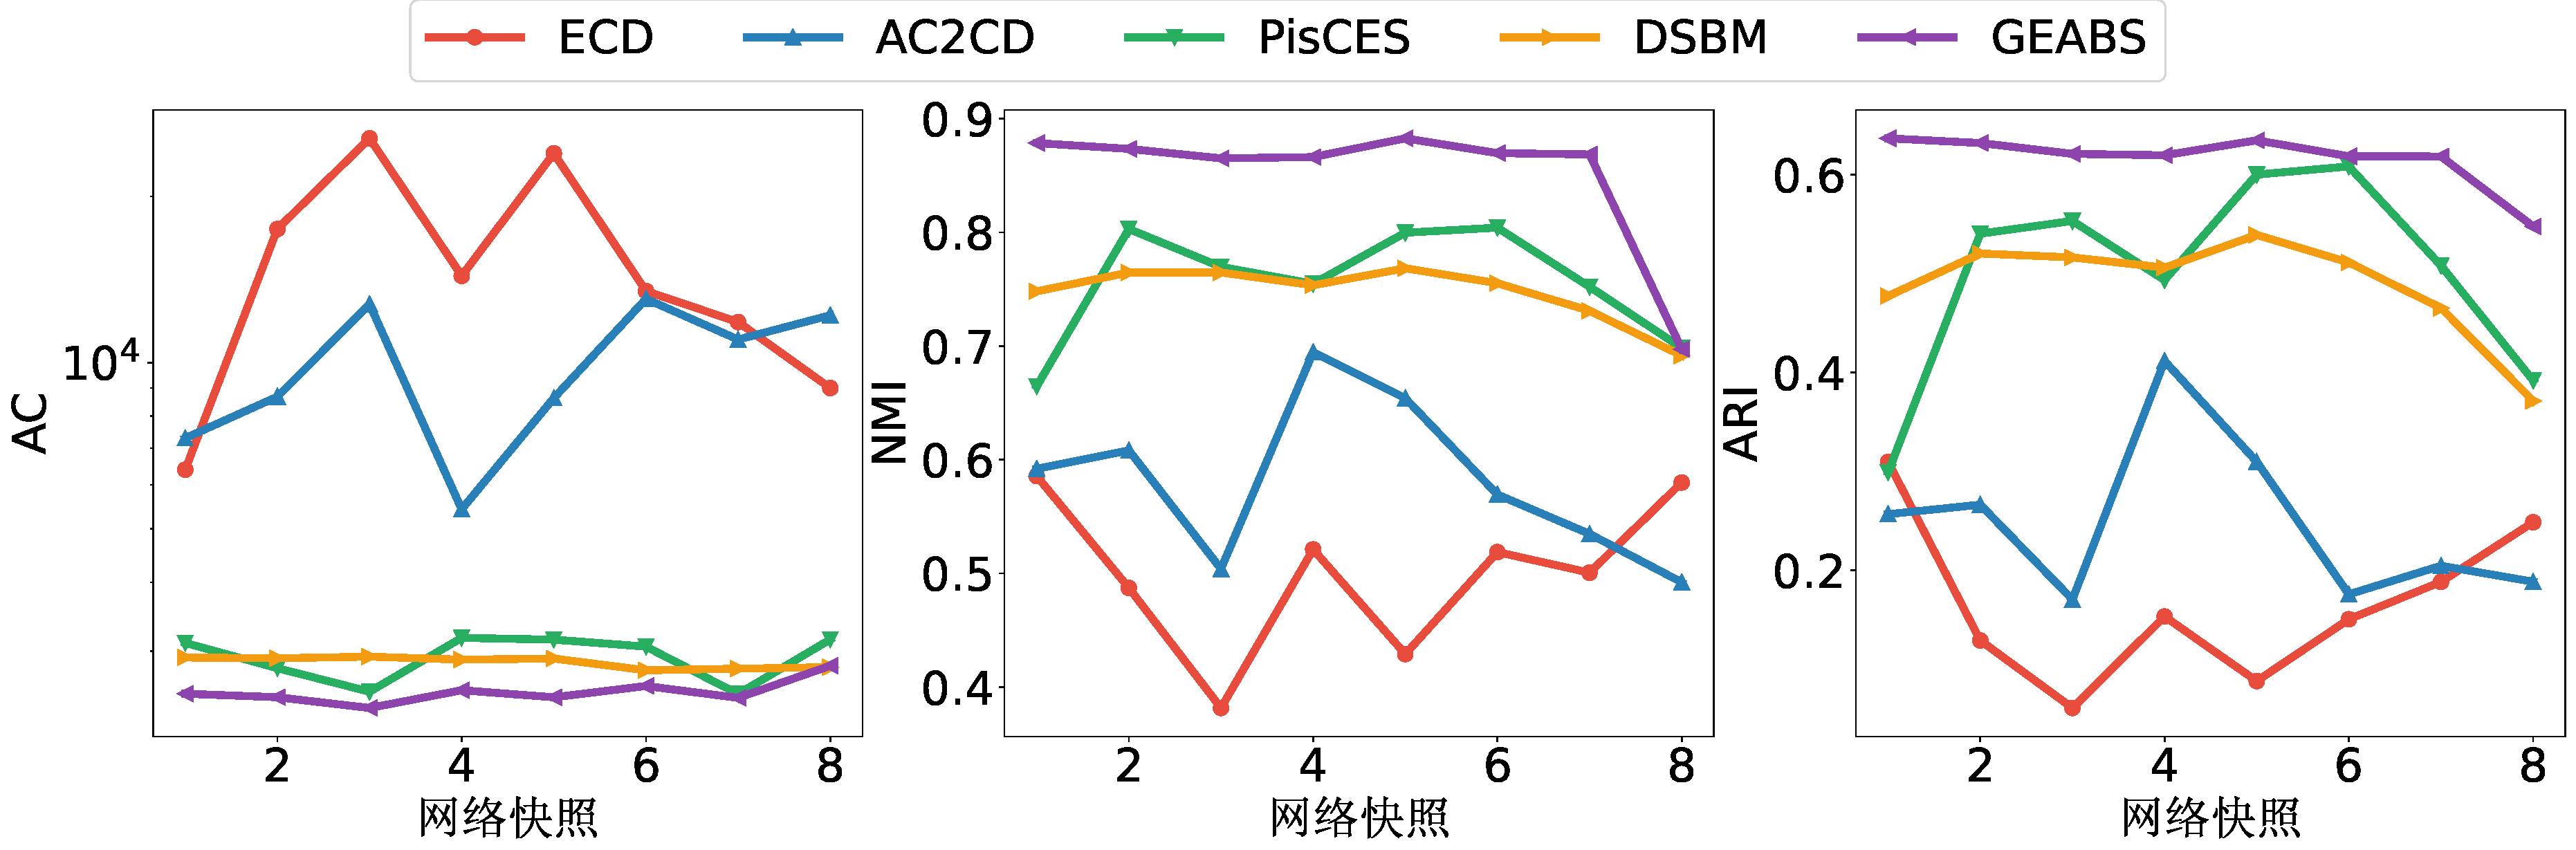
\includegraphics[width=0.9\textwidth]{figures/chap05/chap4Kit-emaili2Communitydetection.pdf}
	\caption{Kit-email数据中的社团检测结果}
	\label{fig4:kit-email}
\end{figure}
\begin{figure}
	\centering
	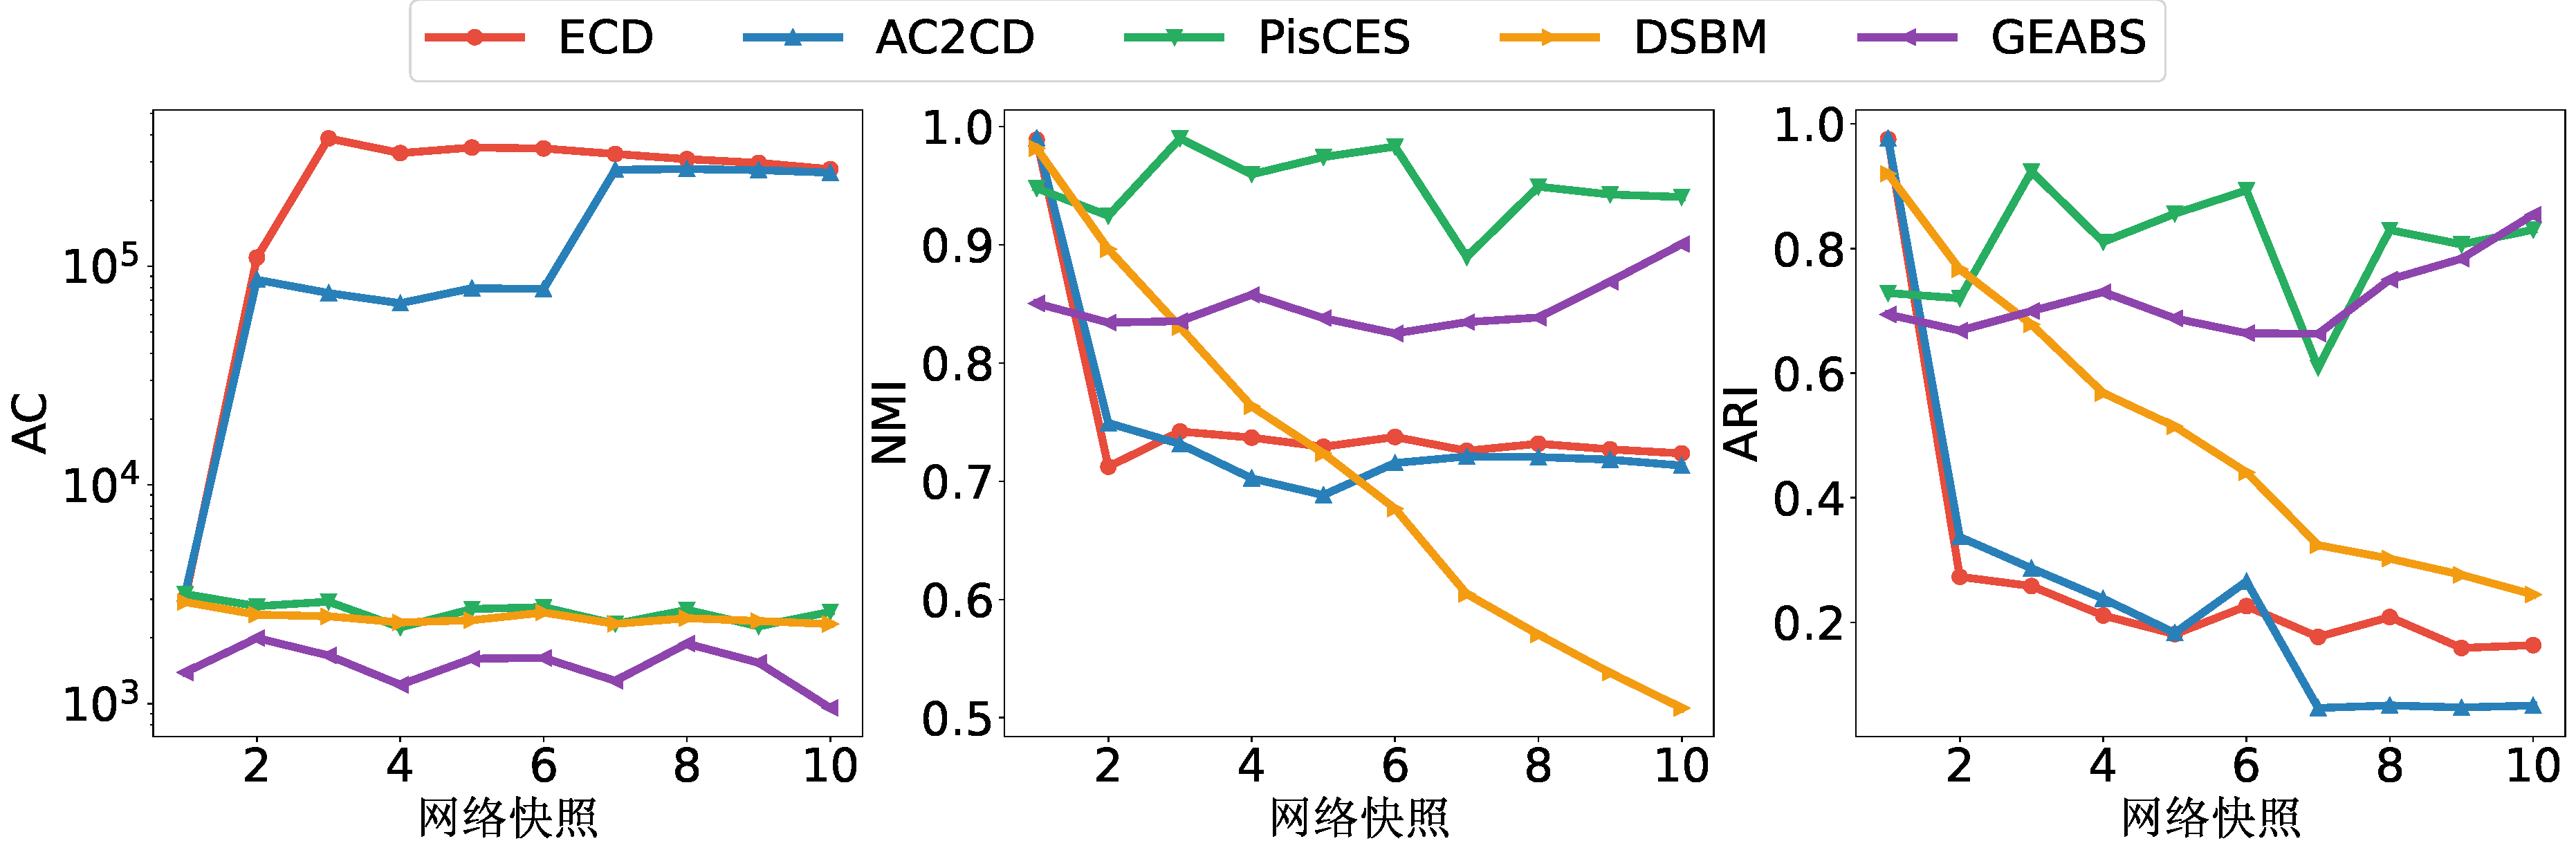
\includegraphics[width=0.9\textwidth]{figures/chap05/chap4mergesplitC.pdf}
	\caption{合成数据中的社团检测结果}
	\label{fig4:mergesplitC}
\end{figure}


 
 
\subsection{快照级别异常检测}

% (1) Network level anomaly
本节基于两个真实世界动态网络数据验证所提出方法GEABS在网络快照级别演化异常(即网络变更点)检测的能力。所用数据集分别为Enron与World Trade网络,二者的网络结构均受到了一定的外部事件影响(如表~\ref{tab:groundE}与表~\ref{tab:groundW}所示),这些外部事件在本部分实验中被视作网络变更点,即网络级别演化异常。为了验证本方法的效果,本节选取$6$个最新且顶尖的动态网络变更点检测算法作为对比方法,包括:

\begin{itemize}
    \item \textbf{SCOUT\cite{hulovatyy2016scout}}:该方法实现了网络变更点和社团的同步检测。它利用现有的搜索策略在时间序列网络中寻找变更点,对同一段内的网络进行聚类,最终通过约束函数找到变化点和社团结构。
    \item \textbf{CICPD\cite{zhu2020change}}:这是一种新颖的基于社团检测的变更点检测方法。它使用PageRank算法学习每个快照的网络表示并计算快照之间的距离,并根据距离度量为边而形成一个新网络。然后对新网络进行谱聚类以检测变更点。
    \item \textbf{GHRG\cite{peel2015detecting}}:这是首个利用在线概率学习框架解决变更点检测的方法,其使用层次随机图生成模型,通过贝叶斯假设检验实现对变更点的量化识别。
    \item \textbf{LAD\cite{huang2020laplacian}}:该方法基于谱优化方法同时检测动态网络的变更点和网络中的事件。LAD的核心思想是通过图拉普拉斯算子的奇异值将整个网络快照映射为低维表示,并显式地建模动态网络演化的短期和长期行为。
    \item \textbf{NetWalk\cite{yu2018netwalk}}:该方法通过学习网络表示来检测动态网络的变更点,并能够随着网络的演化进行动态更新。它通过随机游走将动态网络的节点编码为向量表示,以最小化动态网络中的每个游走节点对的距离作为目标函数,并通过聚类方法实现动态网络的变更点检测。
\end{itemize}


\begin{table}[tp] 
	\centering 
	\fontsize{6.5}{8}\selectfont 
	\begin{threeparttable} 
		\caption{Enron数据集的重要事件(动态网络变更点)} 
		\vspace{0.5em}\centering\wuhao
		\label{tab:groundE} 
		\begin{tabular}{p{1.5cm}p{2cm}p{10cm}} 
			\toprule 
			数据集 & 日期 & 事件 (对应变更点) \\
			\midrule
			&2001-02&Tom White 从 EES 公司辞职\footnote{https://www.agsm.edu.au/bobm/teaching/BE/Enron/timeline.html} \\ 
			
			&2001-04&季度电话会议召开\\ 
			
			\multirow{3}*{Enron} &2001-06&联邦能源管理委员会FERC最终在西部各州实施价格上限。加州能源危机结束。\\ 
			
			&2001-07&Skilling 宣布希望辞职\\ 
			
			&2001-08&Skilling 辞去CEO职务\\ 
			
			&2001-09&Skilling 卖出公司股票\\ 
			
			&2001-11&公司股价暴跌\\ 
			\bottomrule
		\end{tabular}
	\end{threeparttable}  
	\vspace{-2cm}
\end{table}  


\begin{table}[tp] 
	\centering 
	\fontsize{6.5}{8}\selectfont 
	\begin{threeparttable} 
		\caption{World Trade数据集的重要事件(动态网络变更点)} 
		\vspace{0.5em}\centering\wuhao
		\label{tab:groundW} 
		\begin{tabular}{p{1.5cm}p{2cm}p{10cm}} 
			\toprule 
			数据集 & 日期 & 事件 (对应变更点) \\
			\midrule
			&1950&第三次关贸总协定谈判在英国托基举行,各国交换了约 8,700 项关税减让,将 1948 年的关税水平削减了 25\%\\ 
			
			&1955&下一轮贸易谈判于1956年5月完成,关税削减达25亿美元。\\
			
			&1960&欧洲自由贸易联盟(FEAT)成立\\ 
			
			&1964&以已故美国总统的名字命名的肯尼迪回合谈判实现了价值 400 亿美元的世界贸易关税削减。\\ 
			
			\multirow{3}*{World} &1967&欧洲共同体的成立\\ 
			
			\multirow{3}*{Trade} &1968&两项重要的 ISO(国际标准化组织)建议在全球范围内实现了集装箱运输的标准化\\ 
			
			&1971&T护林员委员会成立于 1971 年,旨在为与国际贸易和《不扩散核武器条约》(NOT)有关的核产品的解释提供建议。\\ 
			
			&1973&中东石油危机\\ 
			
			&1983&1983 年,随着中苏关系逐渐缓和,中亚边境贸易恢复。~\cite{karrar2016resumption}\\ 
			
			&1991&苏联解体 \cite{cuaresma2012borders}\\ 
			
			&1999&欧元的诞生影响了欧元区的贸易平衡\\ 
			\bottomrule
		\end{tabular}
	\end{threeparttable}  
	\vspace{-1cm}
\end{table}


\subsubsection{变更点检测的评价指标}

% Change point detection can be used as a binary classification problem, so we can calculate the scores of $Precision$, $Recall$ and ${F_1}$ to evaluate the performance of our model, which are separately defined as:
% \begin{equation}
%     \begin{split}
%         Precision = \frac{TP}{TP + FP},
%     \end{split}
% \end{equation}
% where \emph{Precision} quantifies the number of positive class predictions that actually belong to the positive class. %Its calculation formula is as follows:
% \begin{equation}
%     \begin{split}
%         Recall = \frac{TP}{TP + FN},
%     \end{split}
% \end{equation}
% where \emph{Recall} quantifies the number of positive class predictions made out of all positive examples in the dataset. 
% \begin{equation}
%         F_1 = \frac{2TP}{2TP + FP + FN},
% \end{equation}
% where the comprehensive measurement ${F_1}$ provides a single score that balances both the concerns of precision and recall in one number. %Its calculation formula is as follows:

% These values are in the range of 0 to 1. A score of 1 indicates a perfection spotting of change points, while a score of 0 implies that no change points being detected at the other extreme. The change point in our model is calculated by extracting the local maximum value of $ E_{nl}^{(t)} $. 
网络变更点检测可以被视为一个二元分类问题,因此本章可以计算精度($Precision$)、召回率($Recall$)和${F_1}$值来评估本节涉及的模型的网络演化异常检测效果,其定义分别为:
\begin{equation}
    \begin{split}
        Precision = \frac{TP}{TP + FP},
    \end{split}
\end{equation}
\emph{Precision}量化了被预测为正类的样本中实际属于正类的比例。
\begin{equation}
    \begin{split}
        Recall = \frac{TP}{TP + FN},
    \end{split}
\end{equation}
\emph{Recall}量化了数据集中所有正类样本中被正确预测为正类的比例。
\begin{equation}
        F_1 = \frac{2TP}{2TP + FP + FN},
\end{equation}
${F_1}$提供了平衡精度和召回率的单一指标。

这些值的范围均在$0$到$1$之间。当指标为$1$时,表示该方法检测到了所有网络变更点,反之则表示该方法未检测到任何网络变更点。本章模型中的网络变更点通过提取$E_{nl}^{(t)}$的局部最大值来计算(即当连续快照中的$E_{nl}^{(t)}$变动剧烈时,认为是网络演化异常)。

\subsubsection{网络级别异常检测结果}



\begin{table}[tp]  
	\centering  
	\begin{threeparttable}  
		\caption{GEABS与对比方法在网络演化异常检测中的精度、召回率和F1值对比}  
		\label{tab:performance_comparison}  
		\vspace{0.5em}\centering\wuhao
		\begin{tabular}{p{1.5cm}p{1.5cm}p{1.5cm}p{1.5cm}p{1.5cm}p{1.5cm}p{1.5cm}}
			\toprule  
			\multirow{2}{*}{方法}&  
			\multicolumn{3}{c}{Enron数据集}&\multicolumn{3}{c}{World Trade数据集}\cr  
			\cmidrule(lr){2-4} \cmidrule(lr){5-7}  
			&精度&召回率&${F_1}$&精度&召回率&${F_1}$\cr  
			\midrule  
			SCOUT&{\bf 1.0000}&0.1818&0.3077&0.4000&0.1818&0.2500\cr 
			CICPD&0.5714&0.5714&0.5714&0.3333&0.4545& 0.3846\cr 
			GHRG&0.4284&0.1667&0.2400&0.3500&0.6364&0.4516\cr 
			LAD &0.6667&0.5714&0.6154&0.2222&0.3636&0.2758\cr  
			NetWalk &0.8333&{\bf 0.7143}&0.7692& 0.7333 &0.8181&0.7734\cr  
			GEABS&{\bf 1.0000}& {\bf 0.7143}&{\bf 0.8333}&{\bf 0.7143}&{\bf 0.9091}&{\bf 0.8000}\cr  
			\bottomrule  
		\end{tabular}  
	\end{threeparttable}  
\end{table}
如表~\ref{tab:performance_comparison}所示,本章的方法 GEABS 在所有对比方法中表现最佳。GEABS在Enron数据上的精度为$1$,这表明GEABS找到的所有异常点都是真实的。GEABS在World Trade数据集上的召回率约为$0.91$,这意味着该方法几乎找到了该数据中的所有异常点。值得一提的是,正如图~\ref{fig:enron-net}所示,该图计算了GEABS、NetWalk和LAD在Enron 数据集和World Trade数据集中,前$k$个网络级异常值对异常事件的击中率。由于 World Trade数据集相对复杂,NetWalk和LAD在该数据集中表现不佳。但在 Enron数据集中,NetWalk具有良好的击中率。然而,NetWalk和LAD的前$10$个击中率都低于GEABS。反观GEABS,其在Enron数据集中,前$5$个网络异常的击中率为$100\%$,而在World Trade数据集中,GEABS的前$3$个网络异常值的击中率为$100\%$,这证明了GEABS网络级异常检测方案的有效性和所提出网络演化异常指标的正确性。



%\renewcommand{\arraystretch}{1.5}  
  

\begin{figure}
	\centering
	\subfigure[Enron]{
		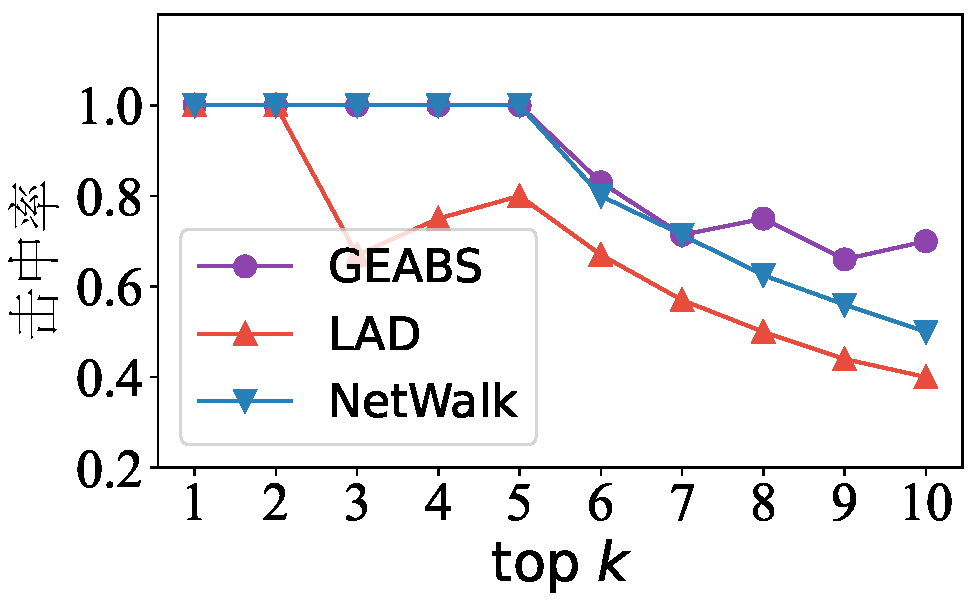
\includegraphics[width=0.4\textwidth]{figures/chap05/nethitrate-enron-new.pdf}}
	\subfigure[World trade]{
		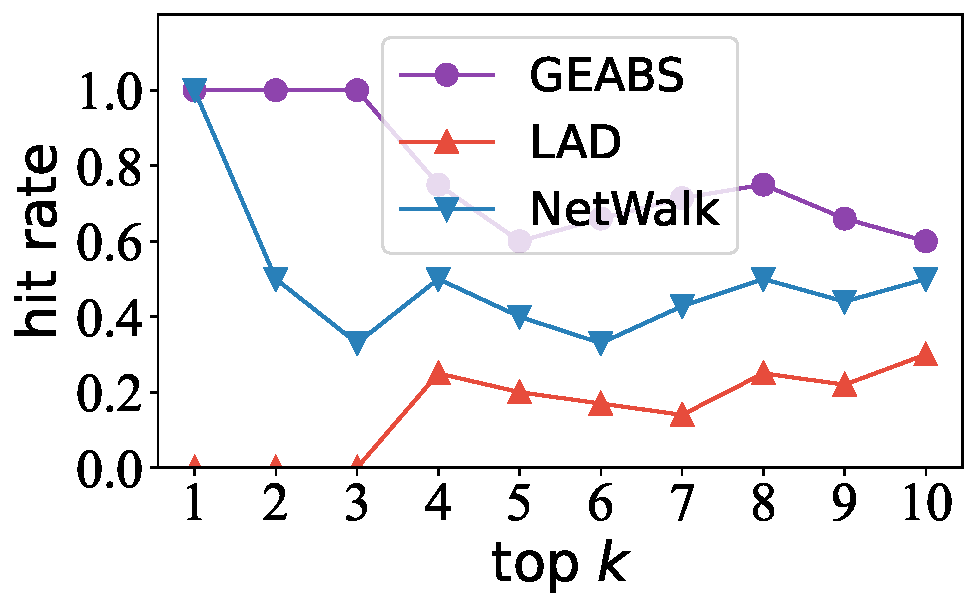
\includegraphics[width=0.4\textwidth]{figures/chap05/nethitrate-World-new.pdf}}
	\caption{GEABS与LAD、NetWalk的网络级别演化异常$top-k$击中率}
	\label{fig:enron-net}
\end{figure}






\subsection{社团级别异常检测}
\label{community anomaly}

\begin{figure}[!htbp]
	\centering
	\subfigure[GroundTruth]{
		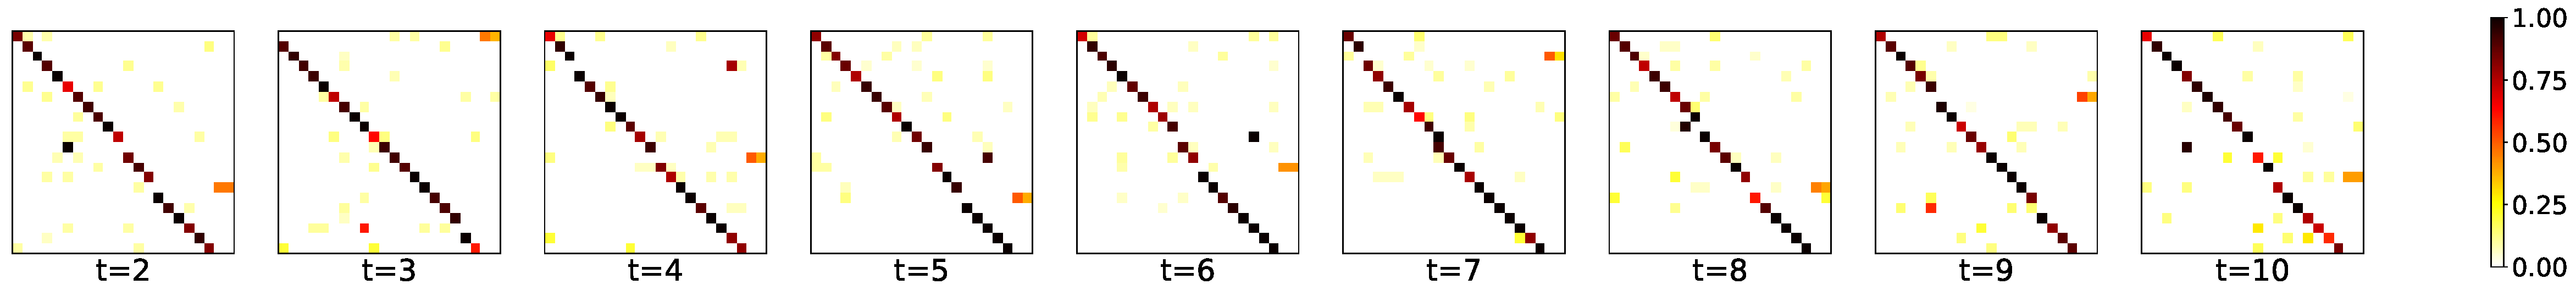
\includegraphics[width=0.7\textwidth]{figures/chap05/mergesplitAGND.pdf}}
	\subfigure[GEABS]{
		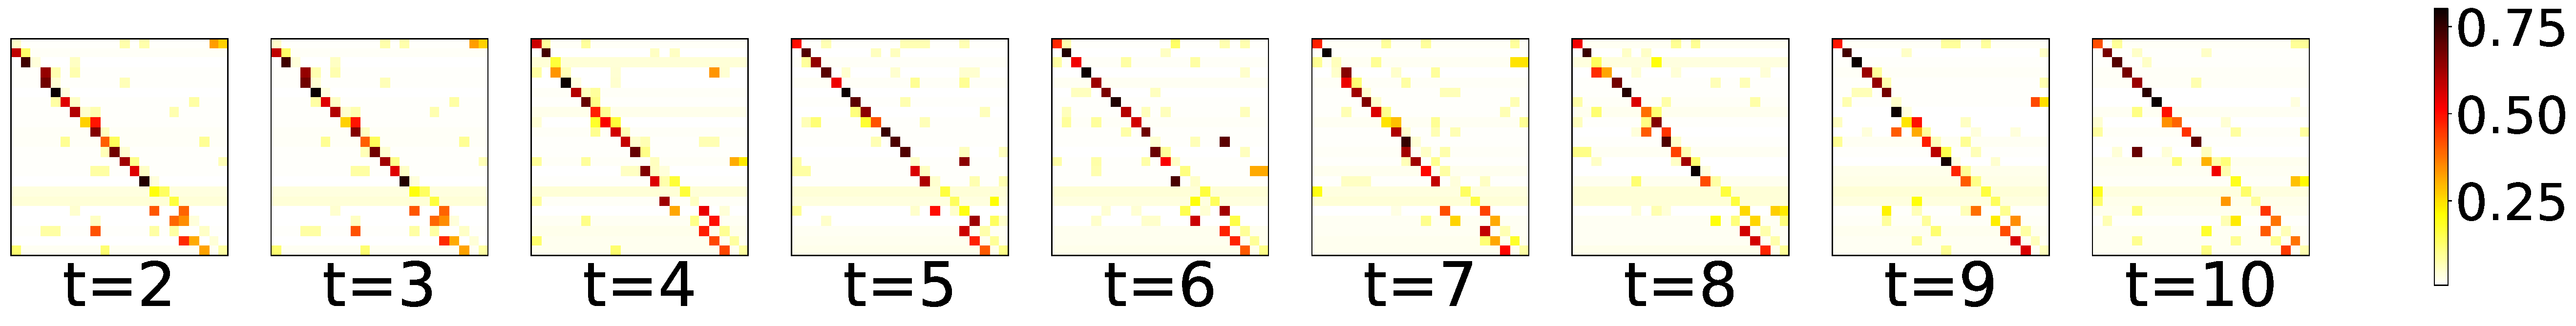
\includegraphics[width=0.7\textwidth]{figures/chap05/mergesplitA.pdf}}
	\subfigure[PisCES]{
		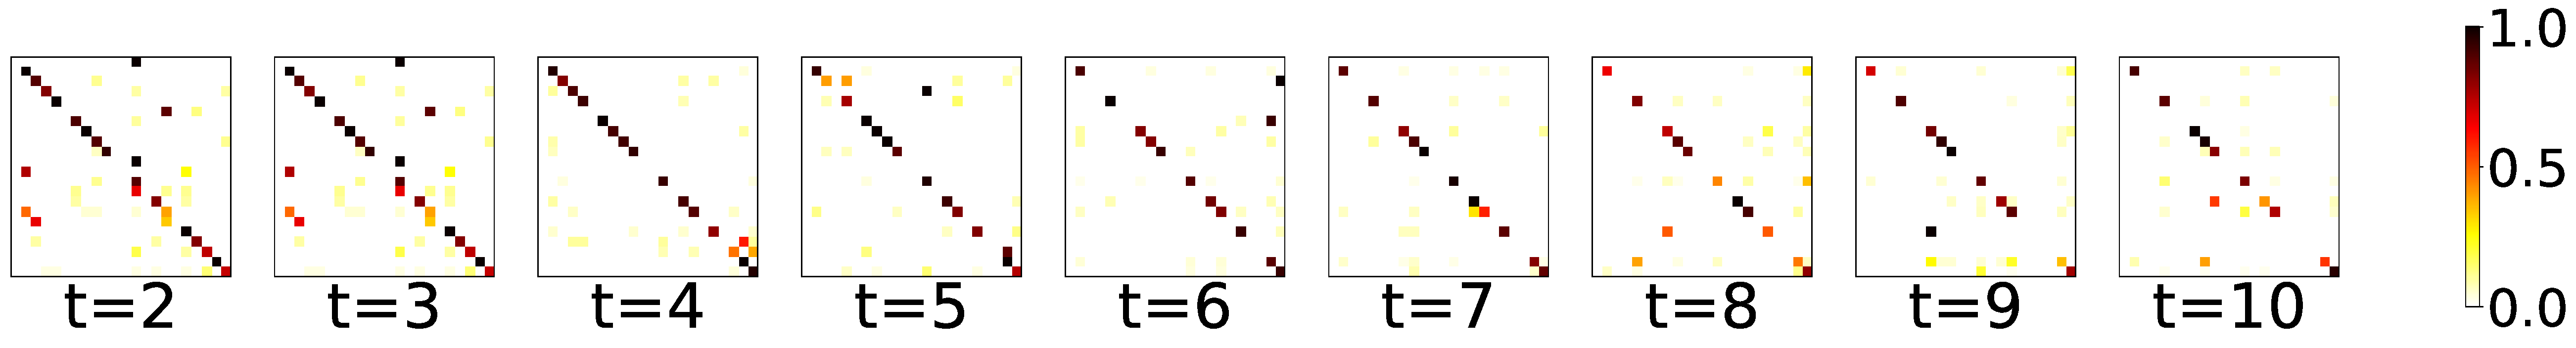
\includegraphics[width=0.7\textwidth]{figures/chap05/mergesplitAPisCES.pdf}}
	\caption{生成数据中的社团转移可视化}
	\label{fig:mergesplitA}
\end{figure}

本章使用生成网络来衡量模型参数$A$对于捕获社团转移倾向的能力,即对社团级别演化异常的刻画能力。本节将模型的转移倾向矩阵$A$与数据集中真实的转移行为以及具有最佳社团检测性能的对比方法PisCES的转移行为进行比较(考虑到动态社团检测效果直接体现了模型对动态网络社团演化的建模能力,故仅与PisCES进行对比),结果如图~\ref{fig:mergesplitA}所示。从该热图可以看出,GEABS能够更好地捕获动态网络中社团的转移倾向,而PisCES所刻画的社团演化则与Ground Truth相差较大。因此,可以看出GEABS可以更好地刻画社团合并、分裂、扩展和收缩等社团事件,因为社团转移矩阵$A$能够准确地捕获社团内节点的未来行为趋势。




另外,GEABS可以处理动态网络中社团数量的变化。在真实网络中,每个快照的社团数量是未知的。社团可能在演化过程中进行合并、分裂或消亡,这些社团级别的演化事件都可能导致社团数量的变化。因此,本节在Enron数据集上测试了GEABS在不同快照下不同社团数量的刻画能力,每个快照的社团数量由静态社团检测方法进行确定。如图~\ref{fig:enronTransA}所示,Enron数据中节点的社团成员转移非常剧烈,社团数量在$t=5,6,7,8,9$中均发生了变化。而与表~\ref{tab:groundE}中Enron公司的重大事件进行对比,可以发现$t=6,7,8,9$快照中存在网络变更点,这表明GEABS能够处理不断变化的社团数量,且可以通过对GEABS中社团数量变化对社团级别异常事件进行有效推断。
 
 \begin{figure}[!htbp]
 	\centering
 	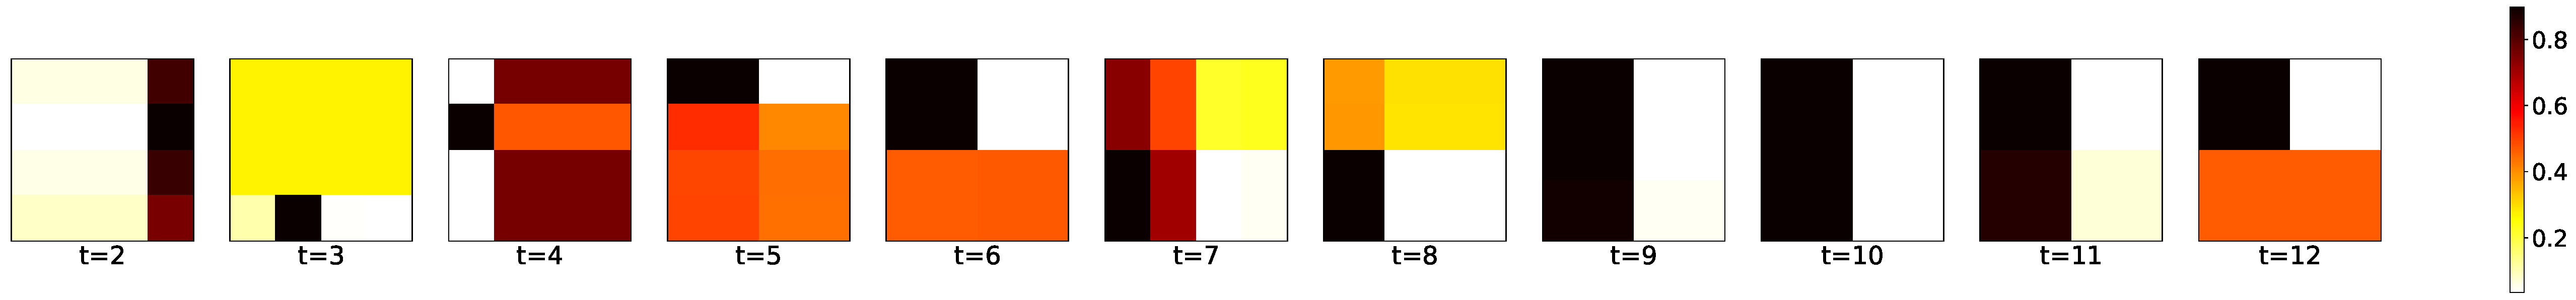
\includegraphics[width=0.7\textwidth]{figures/chap05/EnronTransA-heatmap.pdf}
 	\caption{在不同快照$t$下,GEABS在Enron数据上随社团数量$K$变化的转移矩阵可视化热图}
 	\label{fig:enronTransA}
 \end{figure}
 
 
\subsection{节点级别异常检测}


由于缺乏合理的评价指标和数据集,对节点的异常演化行为很难判断。为评估基于模型参数$\delta$定义的节点异常指数${E_{cl}}_{(i)}$的有效性,本章在World Trade网络中绘制了节点异常指数的散点图,通过世界历史信息启发式地验证参数${E_{cl}}_{(i)}$的合理性。如图~\ref{fig:worldtradenode}所示,红色表示$top-5$异常值最高的国家,绿色节点表示本节手动选出的全球贸易主要国家(包括美国、加拿大、德国、俄罗斯、中国和日本).二战后,美国(USA)是世界上贸易最稳定的国家,也是西方国家的领袖,其节点的异常值达到最低。而日本(JPN)相比其他大多数国家也有较低的异常值,考虑到直到$2000$年,日本的GDP位居世界第二,这也是节点异常指数${E_{cl}}_{(i)}$有效性的一个实例。此外,像海地(HAI)、圣卢西亚(SLU)和多米尼加(DMA)等小国的节点异常值始终较高,通过调研得知,上述国家并没有在国际贸易中具有竞争力的商品,且受到西方制约,这使得这些国家在国际贸易中具有较高的波动性。


\begin{figure}[!htbp]
	\centering
	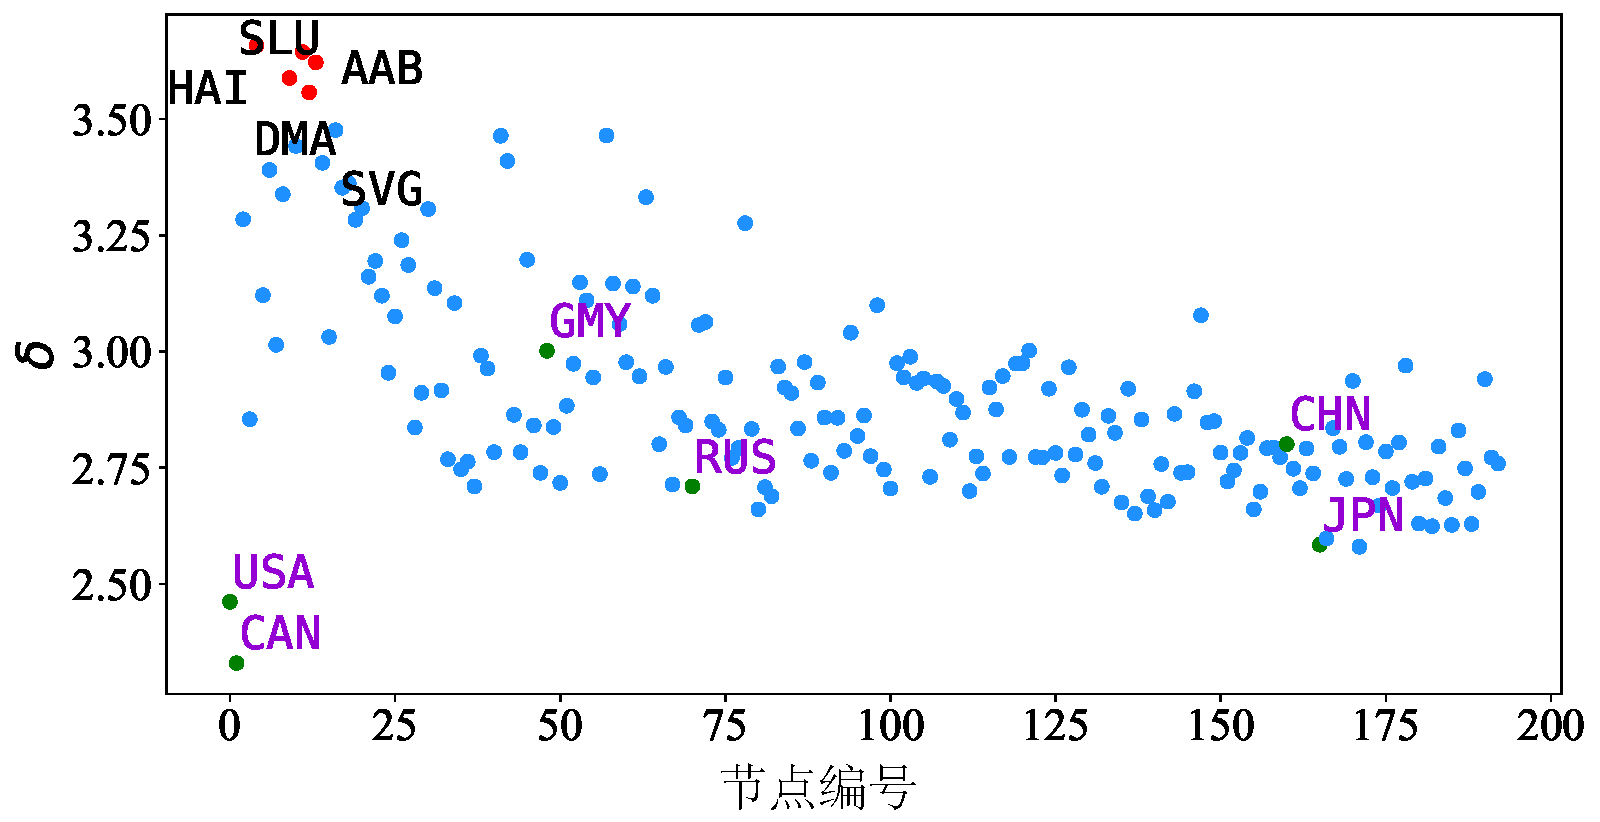
\includegraphics[width=0.6\textwidth]{figures/chap05/worldtradenode-adjusted.pdf}
	\caption{World Trade数据中的节点异常识别结果}
	\label{fig:worldtradenode}
\end{figure}



\subsection{数据挖掘实证}

为了进一步挖掘本模型的演化异常检测能力,本节同时从宏观、微观和介观层面可视化了GEABS模型在国际贸易数据集上检测到的演化异常。如图~\ref{fig:worldtradecaseCN}及图~\ref{fig:worldtradecaseN}所示。其中,图~\ref{fig:worldtradecaseCN}展示了在世界贸易网络中,网络变更点与对应的社团变化之间的关系;而图图~\ref{fig:worldtradecaseN}则展示了对应时间点的异常节点与挑选的核心节点的异常值。从图中可以看出,不同的级别异常指数可能由不同的因素所引起,通过横向与纵向对比,可以有效对动态网络的演化异常进行深入挖掘。例如,在$1950$年,英国举行了关贸总协定(GATT)第三回合谈判,这使得当年有多个国际贸易团体发生合并(社团级别)。而在节点层面,注意到中国(CHN)的$\delta$值非常高,经调研,我国于$1949$年建国,且并未加入国际贸易组织,因而$1950$年的国际贸易并不稳定。$1973$年的石油危机使得俄罗斯的$\delta$值急剧上升。由于俄罗斯的主要出口商品是石油,中东石油危机对俄罗斯的石油出口影响巨大,反而对其他主要国家影响较小。有趣的是,苏联的解体($1991$年)甚至没有影响俄罗斯的进出口贸易(节点层面),但这一事件使得多个国家集团分裂(社团层面)。

\begin{figure}[!htbp]
	\centering
	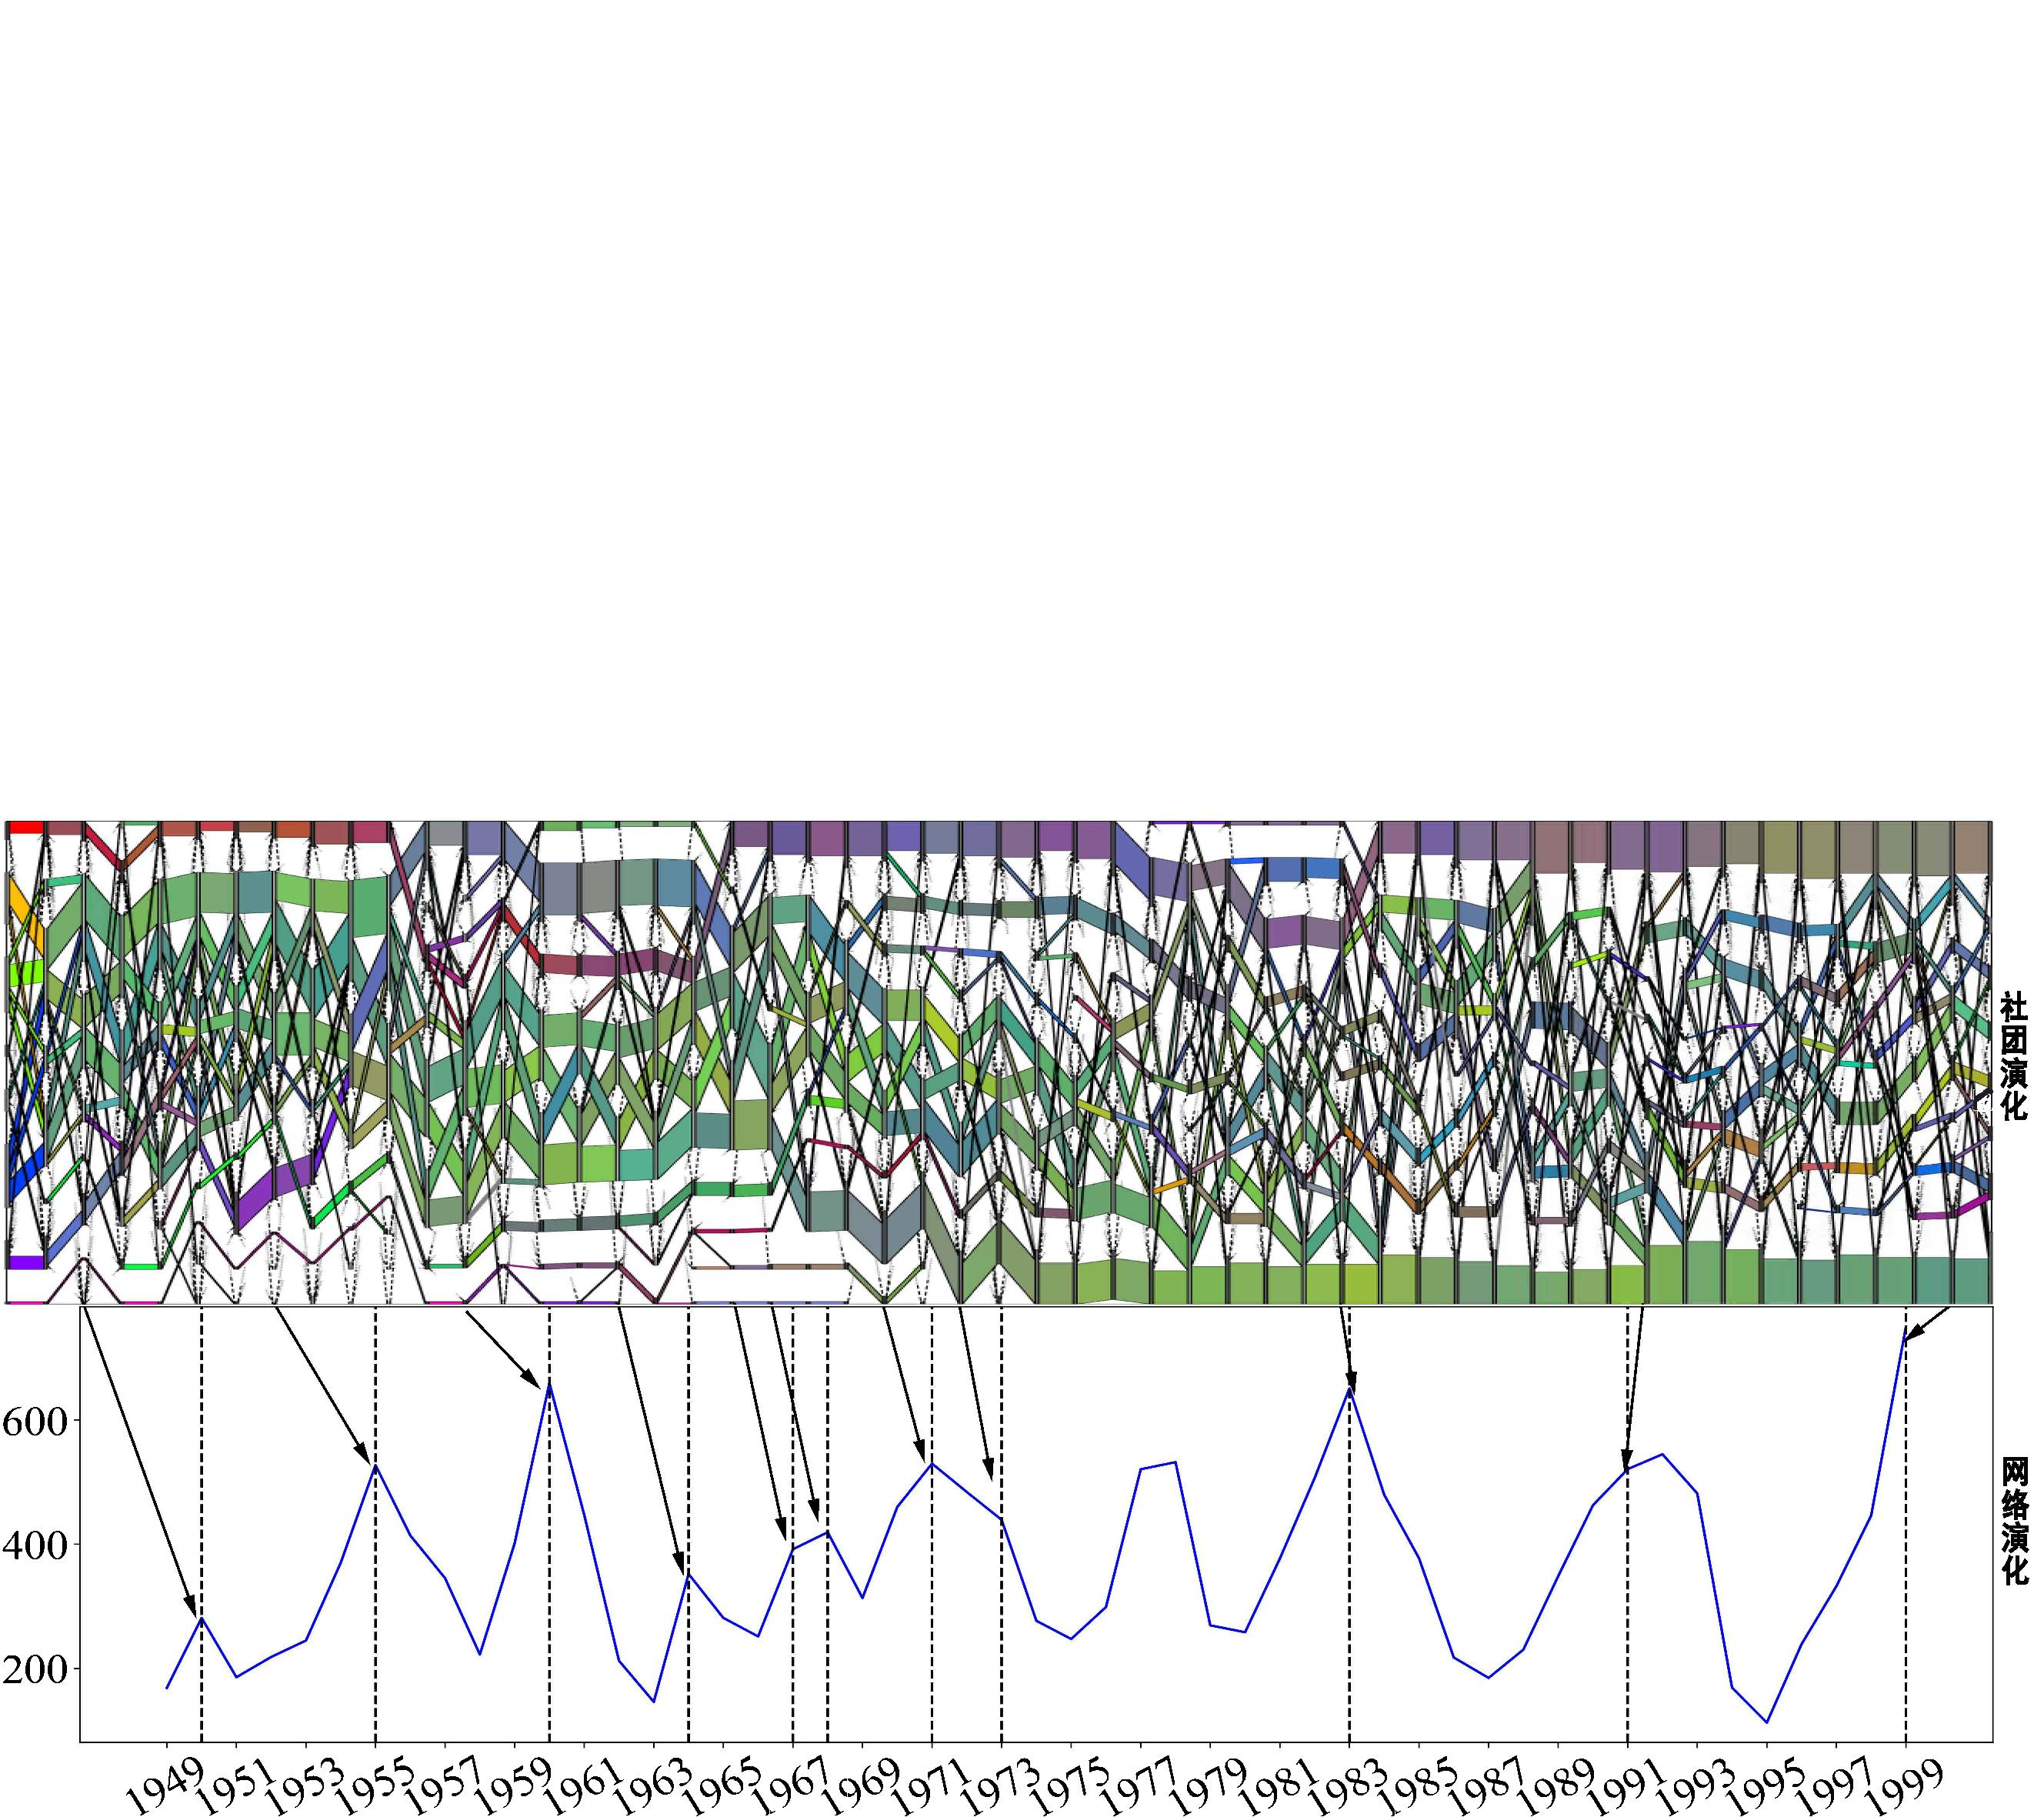
\includegraphics[width=\textwidth]{figures/chap05/worldtrade-CNlevel.pdf}
	\caption{World Trade的层次异常检测案例-社团及网络级别}
	\label{fig:worldtradecaseCN}
%	\vspace{-2cm}
\end{figure}

\begin{figure}[!htbp]
	\centering
	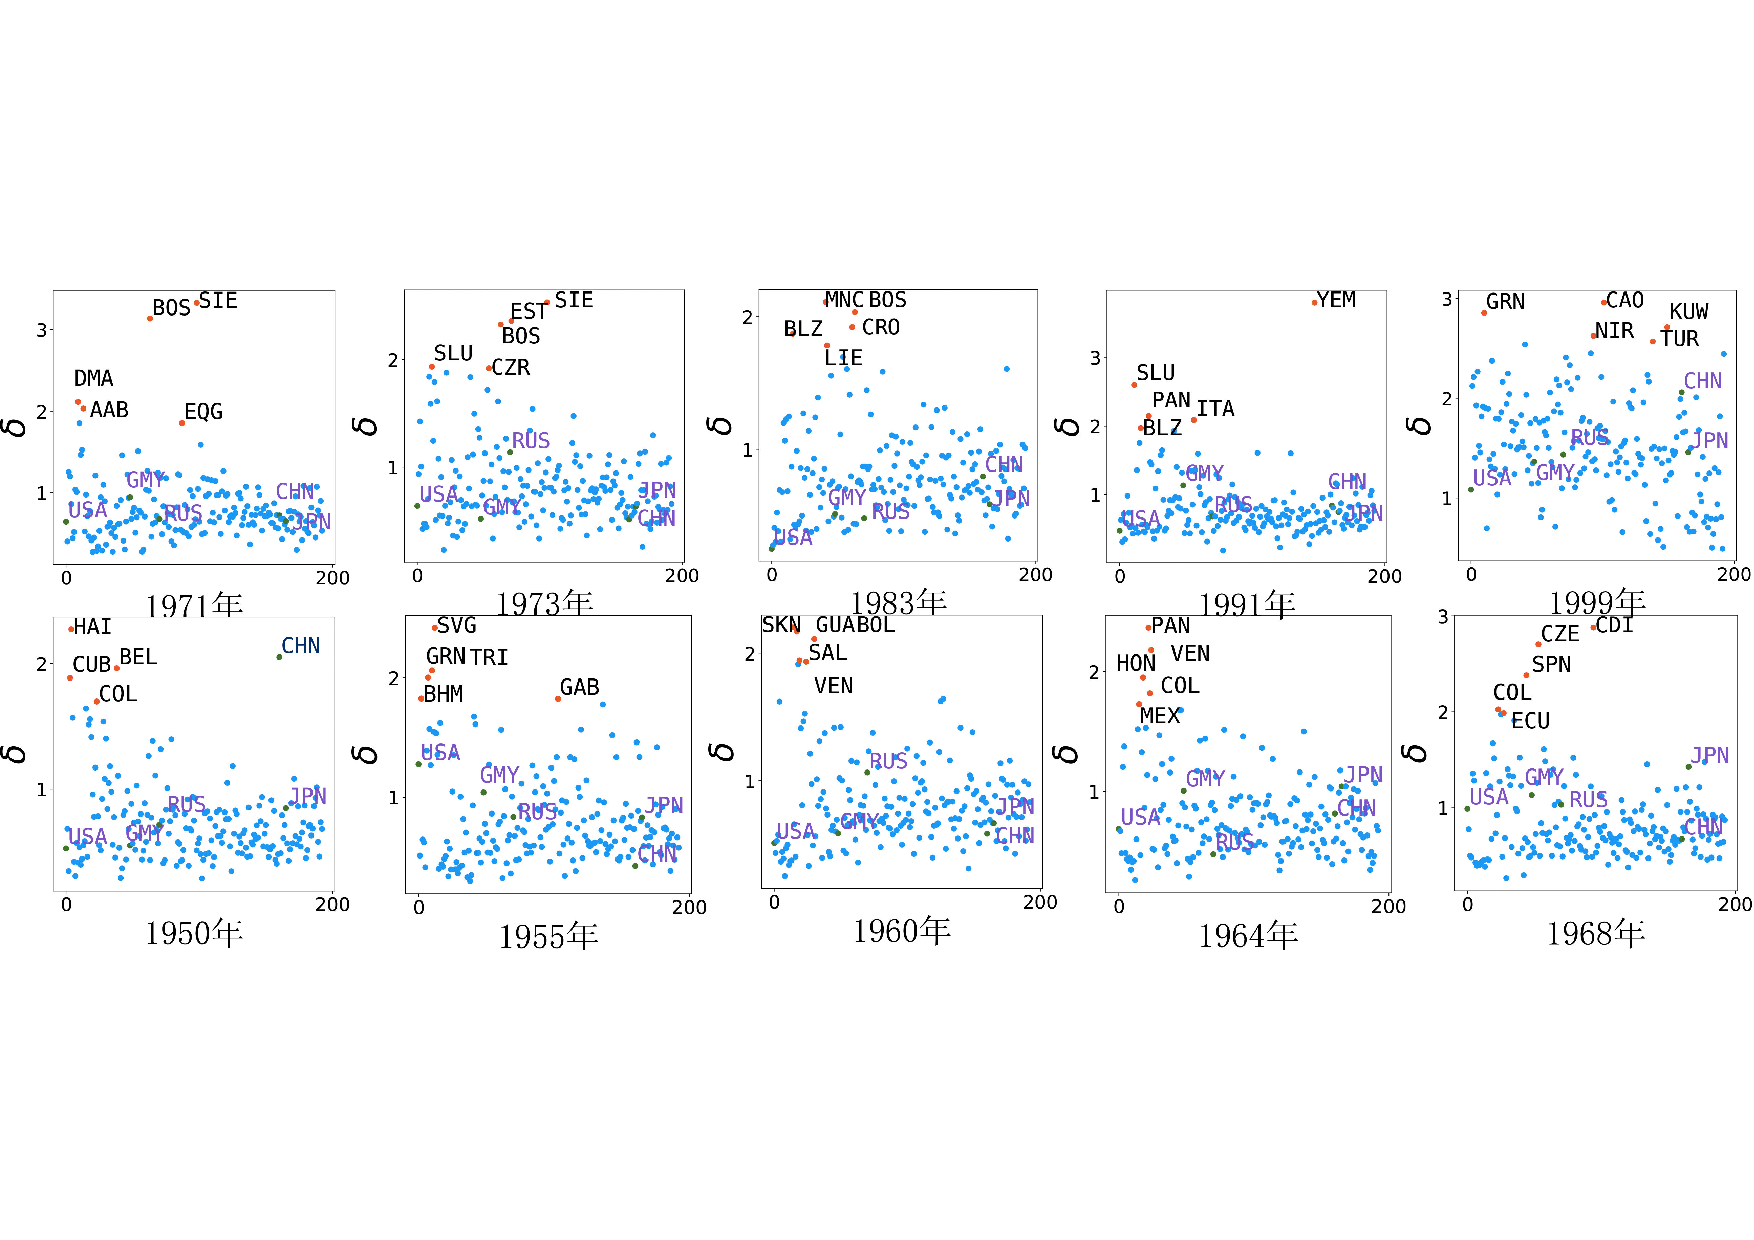
\includegraphics[width=\textwidth]{figures/chap05/worldtrade-Nlevel-new.pdf}
	\caption{World Trade的层次异常检测案例-节点级别}
	\label{fig:worldtradecaseN}
%	\vspace{-2cm}
\end{figure}


另外从图中可以发现,每一次的国际重要事件总会使小国的$\delta$值达到最高。这表明在全球性事件中,小国比大国更易受到影响,这也符合直觉。此外,社团级别的异常和网络级别的异常密切相关,图~\ref{fig:worldtradecaseCN}中的大多数网络变更点都存在社团的重大变化,如$1949$年、$1955$年和$1983$年。然而,节点级别的异常总是受到社团或网络级别的事件影响,例如前文提到的小国节点级沿海异常。这一现象揭示了网络不同层次之间的演化存在更复杂的关系,值得进一步研究。



\section{本章小结\label{chap4:summary}}

本章从动态随机块模型对动态网络建模的能力与演化分析能力出发提出了GEABS生成模型。首先提出了引入节点流行度参数来刻画动态网络中的节点异质性以更好地提升生成模型对动态网络的建模能力;其次提出了基于GEABS不同维度参数的网络-社团-节点不同层次的演化异常检测指标以扩展生成模型在动态网络中的演化分析能力;最后提出了基于变分推断的模型求解方法,利用变分EM方法结合拉格朗日法实现了对模型参数和隐变量的交替更新求解。实验表明,GEABS相较对比方法具有更优的动态网络建模能力,且提出的网络层次演化异常识别参数能够有效地识别动态网络节点、社团与网络快照的演化异常。通过对世界贸易网络World Trade数据集的案例研究也证明了本章所提出的层次演化异常识别指标能够在横向、纵向对比中挖掘动态网络节点、社团、网络快照之间更加复杂的交互依赖关系,能够为动态复杂系统规律挖掘提供有效支撑。

而从模型复杂度角度来看,GEABS具有生成模型的通病,即随着模型设计的精细化,其参数求解效率逐渐下降。虽然可以通过引入负采样、并行计算等方法提升模型的计算效率,但依然难以适用于大规模网络。而能够适用于大规模网络的深度学习方法由于其黑盒特性,难以像生成模型一样有效地支撑对于真实世界的规律挖掘与分析。因此在下一章,本文将提出结合生成模型与深度模型的动态网络建模方法,通过深度生成模型实现网络表示学习与生成模型的有效结合。